
%% For helt almindeligt LaTeX (stabilt): 
%\documentclass{report}

%For RevTeX (Under construction)
%% prl optionen giver referencer på en side for sig selv
%% rmp giver en overskrift til referenceafsnittet, men laver også alle overskriftsfonte om til noget, der ligner nature.
%% notitlepage rykker indholdsfortegnelsen op lige efter abstractet
\documentclass[aps,prb,longbibliography,eqsecnum,a4paper,amssymb,groupedaddress]{revtex4-1}

%Magi kode for at få tocdepth til at virke! nix pille. 
\makeatletter
% Original \l@section:
%\renewcommand*\l@section{\vskip 6pt plus 1pt minus 1pt
%                         \@dottedtocline{1}{1.5em}{2.3em}}
% Modified \l@section:
\renewcommand*\l@section{\ifnum\c@tocdepth>\z@\vskip 6pt plus 1pt minus 1pt \fi
                         \@dottedtocline{1}{1.5em}{2.3em}}
\makeatother

%tocdepth=0 betyder at alle afsnit i klassen under "chapters" ude bliver table of contents (indebærende "sections", "subsections" osv..) 
\setcounter{tocdepth}{0}


\usepackage[usenames, dvipsnames]{color}

\usepackage[utf8]{inputenc}
\usepackage{amsmath}
\usepackage{float}
%\usepackage{natbib}
\usepackage{caption}
\usepackage{subcaption}
\usepackage{graphicx}
\usepackage{hyperref}
\usepackage{siunitx}
%\usepackage[backend=biber]{biblatex}
%\addbibresource{bibliography.bib}
\usepackage{geometry}
 \geometry{
 a4paper,
 total={140mm,227mm},
 left=35mm,
 top=35mm,
 }

%%%%%%%%%%     Egne kommandoer    %%%%%%%%%%%%%
% Vektor
\newcommand{\V}[1]{\mathbf{#1}}

% Ofte brugte felter
\newcommand{\E}{\V{E}}
\newcommand{\B}{\V{B}}
\newcommand{\D}{\V{D}}
\newcommand{\Hf}{\V{H}}

\newcommand{\Red}[1]{\colorbox{Red}{#1}}

%udkommentere store ting
\newcommand{\comment}{}

\begin{document}

\pagenumbering{gobble}

\begin{titlepage}
    \begin{center}
        \vspace*{1cm}
        
        \Huge
        \hline
        \vspace{0.5cm}
        \textbf{Topology Optimisation of Integrated Optical Components}
        \vspace{0.5cm}
        \hline
 
        \vspace{2cm}
        \Large
        \textbf{Frederik Werner Isaksen (s144087) \\
                Magnus Middelboe Søborg-Madsen (s144063) \\
                Roar Nind Steffensen (s144107)} \\
                \\
        \vfill

        \includegraphics[width=12cm]{fig/Kasse40nm.png}
        
        \vspace{0.8cm}
        \Large
        January 2016\\
        Course 34029 Physics Project\\
        BSc Eng Physics and Nanotechnology\\
        Technical University of Denmark\\
        Supervisor: Lars H. Frandsen\\
        \vspace*{0.8cm}
    \end{center}
\end{titlepage}


\section*{Abstract}


This paper describes a somewhat successful attempt at making a silicon-based $2.8 \times 2.8$ \si{\micro m^2} optical broadband wavelength demultiplexer using an inverse design strategy based on topology optimisation. The design goal was to demultiplex an infrared broadband signal into two output signals peaking at 1300 nm and 1550 nm wavelengths, respectively. We obtained six different designs that, in finite-difference time-domain simulations, successfully demultiplexed the signal.
 All six designs had insertion losses (peak transmissions) around $-$0.5 dB and crosstalk around $-$17 dB. However, experiments on fabricated designs did not yield as satisfactory results. The best fabricated design had a peak insertion loss at $-$5 dB in the [1250, 1400] nm range, a peak insertion loss at $-$1 dB in the [1400, 1650] nm range, and peak crosstalk around $-$10 dB. The discrepancy is presumably attributed to a difficult translation from blueprint design to fabrication.



\section*{Acknowledgements}
We would like to thank senior researcher Lars Hagedorn Frandsen for his fantastic supervision and importance in the making of the project.

%tocdepth=1 indstiller toc til normal herefter. 
\addtocontents{toc}{\setcounter{tocdepth}{1}}
\newpage
\tableofcontents
\newpage
\section{Introduction}
\pagenumbering{arabic}
\setcounter{page}{1}
Telecommunications networks depend increasingly on optical components to increase data speed while minimising energy consumption. But photonics still has much unfulfilled potential. \\
\\
The density of transistors in computers has successively followed Moore's law for the past decades, with the consequences of continuously increasing processing speed, but also the number of signal-carrying cables and signal-processing devices. While optical fibres are well-used for long-distance communication, short-distance communication within e.g. computer clusters commonly rely on electrical signals and devices.\\
\\
Optical fibres are used to send signals at light speed with low heat production over large distances at an affordable price. Wavelength-division (de-)multiplexers are used to either split or combine these optical signals, making them a valuable tool in signal processing, especially for short-distance communication. But current wavelength demultiplexers have fairly large footprints, such as IBM's 1-to-8 wavelength (de-)multiplexer \cite{IBMdemultiplexer}, which measures 500 $\times$ 200 \si{\micro m^2}. \\
\\
In this project, we wish to create a 1-to-2 wavelength demultiplexer with a 2.8 $\times$ 2.8 \si{\micro m^2} footprint, more than 12000 times smaller than the (de-)multiplexer from IBM. The demultiplexer must split wavelengths of 1300 nm and 1550 nm into two separate output waveguides. A device with the same goals was previously created at Stanford\cite{Stanford} with an inverse design strategy not relying on topology optimisation. We wish to show that topology optimisation will yield better results in terms of decoupling the signal, as well as improving the insertion loss.\\
\\
The software used in this project was developed by research groups at DTU Photonics and DTU Mechanics. The software simulates transmission of light through a silicon structure, and finds a local solution for the design, given specified objectives and an initial structure. The design goal is achieved through topology optimisation; An inverse design-method relying on Finite-Difference Time-Domain (FDTD) calculations where the silicon structure is iteratively regulated with respect to a specified set of objective functions.

\begin{figure}[h!]
    \centering
    \includegraphics[width=0.7\textwidth]
    {fig/introduction/demultiplexer.pdf}
    \caption{The goal of this project: Creating a wavelength demultiplexer, a device for splitting optical signals, through topology optimisation.}
    \label{fig:my_label}
\end{figure}



\section{Theory}
\subsection{Maxwell's equations}

Electromagnetic waves are a manifestation of oscillations of the space- and time-dependent electromagnetic fields $\E$, $\B$, $\D$ and $\Hf$. We denote the fields by their usual names:
\begin{itemize}
\item[] $\E$ is the electric field.
\item[] $\B$ is the magnetic field.
\item[] $\D$ is the electric displacement.
\item[] $\Hf$ is the auxiliary field (often just called "H").
\end{itemize} 
\\
The behavior of these fields in matter is governed by the Maxwell equations \cite{Griffiths}: 

\begin{align}
\nabla \cdot \D &= \rho_f \\
\nabla \times \E &= -\dfrac{\partial \B}{\partial t} \\
\nabla \cdot \B & = 0 \\
\nabla \times \Hf &= \V{J}_f + \dfrac{\partial \D}{\partial t}
\end{align}

Here $\rho_f$ and $\V{J}_f$ denote the free densities of charge and current, respectively, and $t$ is the time variable. In our case, concerning light propagation through silicon structures, a number of simplifications can be made:
First, we can use the following relations for linear, isotropic and non-dispersive materials \cite{LirongYang}:

\begin{align}
\D &= \epsilon \E \\
\B &= \mu\Hf 
\end{align}

Furthermore, No free charge nor current is present in our structures and hence $\rho_f = 0$ and $\V{J}_f = \V{0}$. Using this information we obtain the following equations \cite{LarsPhD}:


\begin{align}
\nabla \times \E &= -\mu \dfrac{\partial \Hf}{\partial t} \label{Mxeq1}\\
\nabla \times \Hf &= \epsilon \dfrac{\partial \E}{\partial t} \label{Mxeq2}
\end{align}

Thus the problem of determining how light propagates through our structures comes down to determining the fields $\E$ and $\Hf$ by solving the above differential equations.

\subsection{The FDTD method}

The Finite-Difference Time-Domain (FDTD) method is an algorithm for solving the Maxwell equations numerically. The method consists of discretising $\E$ and $\Hf$ into a lattice, setting some initial values and boundary conditions, and then solving a discretised variant of the equations \eqref{Mxeq1} and \eqref{Mxeq2}  one time-step at a time. More information on the method can be found in references \onlinecite{LirongYang,LarsPhD}.
\subsection{Inverse design vs conventional design}

With a conventional design strategy, you first discover (usually in a scientific manner) a property of nature, and then apply this property to produce technology and/or solve a problem. An example of this process is when engineer Percy Spencer in 1945 noticed that microwaves from a radar had melted a chocolate bar in his pocket. This discovery led Spencer to develop the microwave oven \cite{wikiMicrowave}.
With an inverse design strategy, you do the opposite: You set a goal for a final design, a component with a specific set of physical properties, and approach this design by following a set of design principles. Such principles will typically involve a combination of intelligent use of scientific theory, as well as a degree of trial and error. The latter is often called the Edisonian approach. If you greatly systematise the design principles, the inverse strategy can be expressed as an algorithm to a computer. This is the great advantage of inverse design; it can be used to automate and efficiently design products and components to fit consumer needs, and lower the number of constraints set by the designer.

\subsection{Topology optimisation}

Topology optimisation is an inverse design method where an algorithm performs calculations on a mesh region that is initially very simple - in our project, a square box or Y-junction. \texttt{mesh} refers to the discretised lattice of data points representing the silicon structure and its immediate surroundings.
The algorithm then optimises the structure by redistributing material in a \texttt{design domain}, within the \texttt{mesh}. The structure is manipulated to accomplish the goal described in the objective function, while Maxwell's equations are obeyed in every step. Notice that while the algorithm is only allowed to redistribute material in the \texttt{design domain}, Maxwell's equations are obeyed in the larger region, the \texttt{mesh}.

DTU Photonics and DTU Mechanics have developed a topology optimisation software package called PhaZor, which we used to design the demultiplexers described in this paper. Details about using PhaZor are described in the design section. For details about the algorithms, see ref. \onlinecite{PhaZor}.


\section{The design process}
\subsection{The PhaZor script}

To use PhaZor, all details of the task must be included in a \texttt{project.xml} script in order to specify the requested job. \\
\\
The first initial structure is a box-shaped structure with an input waveguide and two output waveguides (Fig.  \ref{fig:stanford}). The \texttt{design domain} is set as the inner box (Fig. \ref{fig:stanford_DD}). \\
\\
The \texttt{design domain} contains the region where the structure is to be optimised, i.e. the input and output waveguides are not changed during optimisation since they are outside the \texttt{design domain}. Since the FDTD method finds local solutions, the final design depends on the choice of initial structure. The \texttt{design domain} and initial structure are given to PhaZor as black and white .png files, with black representing inactive area (empty space) and white representing active area (filled space, in this case Si).\\
\\
The dimensions of the .png files match 1 pixel with 1 nm of the structure. The complete structure is within a defined \texttt{mesh} with a resolution of 40 nm. Each point on the \texttt{mesh} represents the volume encompassing the silicon structure, and these data points are subject to algorithm calculations. The resolution of 40 nm results in a manageable computation time with DTU's HPC cluster, while maintaining a precision high enough to obtain realistic results.\\
\\
The computation time needed to simulate 2D designs is much shorter compared to simulating 3D designs, so the structures were first simulated in 2D, i.e. the components in the \texttt{mesh} region were assumed to have no thickness. The promising structures and parameter values were then used in 3D simulations.\\
\\
The input waveguide is centered at ($-$2710 nm, 0 nm) with respect to the center of the structure, and the output upper and lower waveguides are centered at (2710 nm, 600 nm) and (2710 nm, $-$600 nm), respectively. When moving from 2D to 3D, the structure is given a thickness of 340 nm. The dimensions of structure can be seen on Fig. \ref{fig:initialBox} and Fig. \ref{fig:initialYjunction} (top-down views) and Fig. \ref{fig:initialside} (side-view).\\
\\
In reality the silicon structure is fabricated on a glass (SiO$_2$) surface. This glass surface has to be implemented in the script as well, as its material properties will influence the propagation of light through the demultiplexer component. The minimum feature size of the silicon structure is controlled with a filter size also specified in the script. Each material is defined through their permittivity $\epsilon_r$, permeability $\mu_r$, and conductivity $\sigma_r$, all relative to vacuum. For air; $(\epsilon_r, \, \mu_r, \, \sigma_r)=(1,1,0)$, and for Si; $(\epsilon_r, \, \mu_r, \, \sigma_r)=(11.38,1.0,0)$ in 3D. \\ 

Two Gaussian light pulses are emitted from the input waveguide with specified direction of propagation, temporal width, amplitude, and polarisation (in our case: TE-polarised). Since the optimisation depends on how these two light pulses propagate, the temporal width must be chosen so that the spectral width of the pulses overlap slightly. The optimised structure must able to handle the full spectrum of wavelengths, at least in the [1250, 1650] nm range.
\\\\

\begin{figure}[t]
    \centering
    \begin{subfigure}[h]{0.48\textwidth}
        \centering
        \includegraphics[width=\textwidth]
        {fig/design/stanford.pdf}
        \caption{Initial box-shaped silicon structure.}
        \label{fig:stanford}
    \end{subfigure}
    \hspace{1mm}
    \begin{subfigure}[h]{0.48\textwidth}
        \centering
        \includegraphics[width=\textwidth]
        {fig/design/stanford_Yjunction.pdf}
    \caption{Initial Y-junction-shaped silicon structure.}
    \label{stanford_Yjunction}
    \end{subfigure}
    \caption{The .png images loaded into PhaZor for the box structure and Y-junction structure. For dimensions of the structures (top-down view), see Fig. \ref{fig:initialBox} and Fig. \ref{fig:initialYjunction}. For a side-view, see Fig. \ref{fig:initialside}.}
    \label{fig:Inputfiles}
\end{figure}

\begin{figure}[h]
    \centering
    \includegraphics[width=0.48\textwidth]
        {fig/design/stanford_DD.pdf}
        \caption{\texttt{design domain} for all initial structures.}
        \label{fig:stanford_DD}
\end{figure}


\subsection{Chosen initial structures}
We chose to optimise six initial structures: Three box structures (Fig. \ref{fig:initialBox}), and three Y-junction structures (Fig. \ref{fig:initialYjunction}). The box-shaped design is meant to be the simplest initial design. Furthermore this design is what Stanford used as their initial design \cite{Stanford}, and in order to check our approach compared to theirs, this is the best suited initial design for that purpose. The solutions from the box-shaped structures all turned out to resemble Y-junctions, so by choosing a Y-junction shape as an alternative initial design, we might get closer to a global solution. \\

The three box structures had identical dimensions at start (0th iteration), but were optimised with different filters, i.e. the smallest allowed features on the final design were limited to 40 nm, 60 nm, and 80 nm, respectively.\\

We chose similar Y-junction structures with identical dimensions at the 0th iteration. Likewise, the smallest allowed features were limited to 40 nm, 60 nm, and 80 nm, respectively. From this page onwards, "Box 40 nm" refers to a box-shaped silicon structure with a minimum feature size of 40 nm. Similar names apply to other structures: "Y-junction 80 nm" refers to a Y-junction-shaped silicon structure with a minimum feature size of 80 nm. The structure dimensions remain as expressed in Fig. \ref{fig:initialBox} and Fig. \ref{fig:initialYjunction}.

\begin{figure}[h!]
    \centering
    \includegraphics[width=0.7\textwidth]
    {fig/design/initialBox.pdf}
    \caption{Initial box structure dimensions, top-down view. The \texttt{design domain} is bordered by the dashed line.}
    \label{fig:initialBox}
\end{figure}

\begin{figure}[h!]
    \centering
    \includegraphics[width=0.7\textwidth]
    {fig/design/initialYjunction.pdf}
    \caption{Initial Y-junction structure dimensions, top-down view. The \texttt{design domain} bordered by the dashed line is the same as in the box structure, letting the software add silicon around the Y-junction and thereby not restricting the final structure to the dimensions of our initial structure.}
    \label{fig:initialYjunction}
\end{figure}

\begin{figure}[h!]
    \centering
    \includegraphics[width=0.7\textwidth]
    {fig/design/initialside.pdf}
    \caption{Initial structure dimensions, side-view. Left: input waveguide. Center: Demultiplexer, with an initial structure as a box or Y-junction. Right: Output waveguides.}
    \label{fig:initialside}
\end{figure}

\subsection{Objective functions}
When optimising a structure through the FDTD method with PhaZor, the user must choose an objective. The overall goal is clear: Demultiplex wavelengths of 1300 nm and 1550 nm into two separate output terminals while keeping their Gaussian form. But which objective best describes this goal? The objectives are communicated to PhaZor using \texttt{objective functions}. We used two such functions. The light sources implemented were two Gaussian pulses separated in time; a pulse centered at 1300 nm peaking at $t_1= 50$ fs, and a pulse centered at 1550 nm peaking at $t_2 = 1050$ fs, both with standard deviation $\sigma=\SI{10}{fs}$. We requested a structure that directed the entire pulse excited at $t_1$ to the upper output waveguide, and the entire pulse excited at $t_2$ to the lower output waveguide, see Fig. \ref{fig:initialBox}. While the pulses are separated in time during the optimisation for computational reasons, the fabricated structure can physically handle simultaneous pulses. While the goal seems straight-forward, we employed two very different approaches:\\

\textbf{The objective function \texttt{PointCustom SignalShape}} optimises for a Gaussian pulse with a certain amplitude $A$, peak time $t_0$, and temporal width $T$. This allows us to optimise for the first pulse (1300 nm) in the upper waveguide and second pulse (1550 nm) in the lower waveguide, as illustrated in Fig. \ref{fig:objectiveFunctionGaussian}. We set $A=0.1350$ (arbitrary units) and $t_0=\SI{128}{fs}$ 1580 nm into the upper waveguide and correspondingly $A=0.1235$ and $t_0 = \SI{1128}{fs}$ in the lower waveguide; for both waveguides, we set $T = 10$ fs. These values were obtained from running simulations in a \SI{8000}{nm} long waveguide (equal to the length of our demultiplexer structure) and recording the pulses at the corresponding position. This method yielded mediocre results, perhaps because the pulses tend to be delayed when traveling through the demultiplexer rather than an empty waveguide. The fact that the algorithm has to optimise for many constraints may also have been an obstacle. \\

\begin{figure}[h!]
    \centering
    \includegraphics[width=1.0\textwidth]
    {fig/design/objectivefunctionsgaussian.pdf}
    \caption{When using the objective function \texttt{PointCustom SignalShape}, the main goal is the amplitude, peak time, and temporal shape of the output signals. The pulse sent at $t=0$ has a peak wavelength at 1300 nm. The pulse sent at $t= 1000$ fs has a peak wavelength at 1550 nm.}
    \label{fig:objectiveFunctionGaussian}
\end{figure}

\vspace{1cm}

\textbf{The objective function} \texttt{PointEnergyDensity}
optimises for a Gaussian power spectrum at a specified location with a given peak frequency $\nu$ and spectral width $d\nu$. We optimised for $\nu = 230.0$ THz ($\lambda =$ 1300 nm) and $ \nu= 193.4$ THz ($\lambda =$ 1550 nm) into the upper and lower output waveguide, respectively, and set $d\nu = 9.5$ THz for both waveguides. This is illustrated in Fig. \ref{fig:objectiveFunctionPED}.
This gave much better results. In hindsight, it makes sense: In each iteration, the structure is altered so that more power is delivered to e.g. the upper output, without specifying \textit{when} the signal should arrive. This may lead to odd signal shapes during the optimisation due to unpredictably bad local solutions, but after many (say, $\approx 70$) iterations, a good local solution has been obtained: a structure that splits wavelengths of 1300 nm and 1550 nm into two separate output terminals while keeping their Gaussian form.
 
\vspace{1cm}
 
\begin{figure}[h!]
    \centering
    \includegraphics[width=1.0\textwidth]
    {fig/design/objectivefunctionsped.pdf}
    \caption{When using the objective function \texttt{PointEnergyDensity}, the main goal is optimising power at a specified spectral range. The pulse sent at $t=0$ has a peak wavelength at 1300 nm. The pulse sent at $t= 1000$ fs has a peak wavelength at 1550 nm.}
    \label{fig:objectiveFunctionPED}
\end{figure}
\vspace{1cm}

\subsection{Filter sizes}

In the PhaZor script, the filter size (more specifically, the  \texttt{filter radius}) is specified. This filter size limits the minimum feature size of which the software is allowed to redistribute material. Phazor uses preset sensitivity parameters to control whether material should stay or be moved. The filter starts out very light, letting the structure contain data points with properties between those of Si and air. Throughout the time steps, the filter strength increases exponentially, limiting the amount of material composed partially of Si and air, resulting in a structure mainly with data points representing pure Si or air. \\

The initial areas composed of a mixture of Si and air is visualised as a shaded area with the nuance describing the concentration level of Si. If the filter size is too large, meaning the task set by the objective functions cannot be fulfilled, the resulting design will still have shaded areas, because of the sensitivity and importance of these areas.
\vspace{1cm}


\section{Structures}
The structures that were initially box-shaped, with filter sizes 40 nm, 60 nm and 80 nm, respectively, are shown in Fig. \ref{fig:BoxStructures}, and  the initially Y-junction-shaped structures, also with filter sizes 40 nm, 60 nm and 80 nm, respectively, are shown in Fig. \ref{fig:Y-juncStructures}. As mentioned in the "Filter size" subsection, we see that the designs are not without shaded areas. This is especially true for the structures with larger filter sizes. \\

\subsection{Fabricating the designs}
The fabrication is executed using spin coating, resists, electron beam lithography (e-beam), chemical vapor deposition (CVD), and etching. The designs were fabricated by Lars Hagedorn Frandsen from DTU Photonics \cite{Fabrication}. Since the e-beam removes material from top to bottom chronically, it is not possible to fabricate homogeneous columns of specific concentration of Si and air without a very advanced O$_2$ doping process. Therefore the shaded areas must be converted to black and white, and consequently treated binarily as silicon or air.\\

This is done with a threshold value for silicon concentration, deciding if the area is set to silicon or air. Since the shaded areas are important to the efficiency of the design, forcing the the shaded area into either black or white will sadly lead to a downgrade in performance. The minimum possible feature sizes written with e-beam is around 20 nm \cite{DanchipOfficial}, making it is possible to fabricate structures with a filter size of 40 nm. As seen in Fig. \ref{fig:BoxStructures}, the fabricated structures with feature size 40 nm were remarkably close to the simulated structures.

\newpage

 \subsection{Box structures}

 \begin{figure}[H]
    \centering
    \includegraphics[trim= 8.35cm 2.73cm 8.35cm 2.73cm,clip,width=\textwidth]{fig/boxstructures.pdf}
    \vspace{-2cm}
    \caption{Box structures. Fabrication flaws are evident across all feature sizes, although one would expect the small feature sizes to have more errors due to the higher precision needed. This is due to the fact that a larger feature size also have larger shaded regions, which were not possible to fabricate with our fabrication process. PhaZor uses shaded (grey) pixels to represent materials with property values between silicium and air. In each iteration step, less shading is permitted. When fabricating the structures shown to the left, the coloring is converted to binary: material is either removed (black) or kept (white).}
    \label{fig:BoxStructures}
 \end{figure}

 \newpage
 \subsection{Y-junction structures}
 \begin{figure}[H]
    \centering
    \includegraphics[trim= 8.35cm 2.73cm 8.35cm 2.73cm,clip,width=\textwidth]{fig/yjunctionstructures.pdf}
        \vspace{-2cm}
    \caption{Y-junction structures. Fabrication flaws are evident across all feature sizes, although one would expect the small feature sizes to have more errors due to the higher precision needed. This is due to the fact that a larger feature size also have larger shaded regions, which were not possible to fabricate with our fabrication process. PhaZor uses shaded (grey) pixels to represent materials with property values between silicium and air. In each iteration step, less shading is permitted. When fabricating the structures shown to the left, the coloring is converted to binary: material is either removed (black) or kept (white). PhaZor added material in the initially material-void regions, so the outer edges of the structure no longer outline (simple) Y-junctions.}
    \label{fig:Y-juncStructures}
\end{figure}

 \newpage

\section{Simulation results}

Using PhaZor, the six designs have been simulated, and the transmissions are normalised with respect to a reference waveguide. The results are shown in Fig. \ref{fig:simplots}.
\vspace{-0.1mm}
\begin{figure}[H]
\begin{subfigure}[h]{0.50\textwidth}
        \centering
        \includegraphics[width=1.0\textwidth]
        {fig/simplots/Kasse40nmsimplot.pdf}
        \caption{Simulated transmission through the box structure with feature size 40 nm.}
        \label{fig:transmissionkilde3_a}
    \end{subfigure}%
    ~ 
    \begin{subfigure}[h]{0.50\textwidth}
        \centering
        \includegraphics[width=1.0\textwidth]
        {fig/simplots/Yjunc40nmsimplot.pdf}
        \caption{Simulated transmission through the Y-junction structure with feature size 40 nm.}
    \end{subfigure}
    
    \vspace{5 mm}
    
    
    \begin{subfigure}[h]{0.50\textwidth}
        \centering
        \includegraphics[width=1.0\textwidth]
        {fig/simplots/Kasse60nmsimplot.pdf}
        \caption{Simulated transmission through the box structure with feature size 60 nm.}
    \end{subfigure}%
    ~ 
    \begin{subfigure}[h]{0.50\textwidth}
        \centering
        \includegraphics[width=1.0\textwidth]
        {fig/simplots/Yjunc60nmsimplot.pdf}
        \caption{Simulated transmission through the Y-junction structure with feature size 60 nm.}
    \end{subfigure}
    
    \vspace{5 mm}
    
    \begin{subfigure}[h]{0.5\textwidth}
        \centering
        \includegraphics[width=1.0\textwidth]
        {fig/simplots/Kasse80nmsimplot.pdf}
        \caption{Simulated transmission through the box structure with feature size 80 nm.}
    \end{subfigure}%
    ~ 
    \begin{subfigure}[h]{0.50\textwidth}
        \centering
        \includegraphics[width=1.0\textwidth]
        {fig/simplots/Yjunc80nmsimplot.pdf}
        \caption{Simulated transmission through the Y-junction structure with feature size 80 nm.}
    \end{subfigure}

    \caption{Simulation experiment results. Black: Upper output waveguide. Red: Lower output waveguide. Almost all designs have peak insertion losses at around $-0.5$ dB. For most structures, we see the intercept between the signal graphs at 1420-1422 nm wavelengths. Crosstalk is maximally around $-7$ dB, but much lower through most of the spectrum.}
   \label{fig:simplots}
    
\end{figure}

\newpage

The simulation results look very promising. Almost all designs have peak insertion losses around $-0.8$ dB or better. For all six structures, the transmission graphs intercept at [1420, 1422] nm, i.e. the [1250, 1400] nm spectrum is well separated from the [1400, 1650] nm spectrum. \\
\\
Heuristically, the box structures perform more consistently than the Y-junction structures, but if one were to demultiplex a signal consisting mainly of the [1250, 1300] nm and [1600, 1650] nm light, the Y-junction structures offer insertion losses of $-1$ dB or better, while maintaining cross talks at $-20$ dB.\\
\\
Crosstalk peaks around $-7$ dB, but through most of the spectrum crosstalk is much lower. While $-7$ dB may not seem like a terrific value for crosstalk transmission, it the interesting metric is the difference between the insertion loss and crosstalk transmissions - and here, our structures generally offer a $-6$ dB difference between insertion loss and peak crosstalk, and commonly a difference of -15 dB between insertion loss and crosstalk transmission. The simulation results are summarised in Table \ref{simtable}.


\begin{table}[h!]
\centering
        \begin{tabular}{|l|c|c|c|c|c|c|}
    \hline
    Structure                    & \textbf{Box} & \textbf{Box} & \textbf{Box} & \textbf{Y-junction} & \textbf{Y-junction} & \textbf{Y-junction} \\ 
    Feature size                    & \textbf{40 nm} & \textbf{60 nm} & \textbf{80 nm} & \textbf{40 nm} & \textbf{60 nm} & \textbf{80 nm} \\ \hline
    Peak insertion loss  & $-0.34$ dB  & $-0.64$ dB  & $-0.79$ dB  & $-$0.72 dB         & $-$0.83 dB         & $-$0.74 dB         \\
    (upper output)       & ~         & ~         & ~         & ~                & ~                & ~                \\ \hline
    Peak insertion loss  & $-$0.32 dB  & $-$0.48 dB  & $-$0.49 dB  & $-$0.24 dB         & $-$0.30 dB         & $-$0.45 dB         \\
    (lower output)       & ~         & ~         & ~         & ~                & ~                & ~                \\ \hline
    Peak crosstalk & $-$7.52 dB  & $-$5.41 dB  & $-$5.62 dB  & $-$7.14 dB         & $-$7.31 dB         & $-$7.08 dB         \\
    at wavelength         & 1420 nm   & 1420 nm   & 1421 nm   & 1421 nm          & 1421 nm            & 1419 nm            \\ \hline
    Crosstalk  & $-$20.79 dB & $-$19.53 dB & $-$18.16 dB & $-$23.21 dB        & $-$18.80 dB        & $-$17.67 dB        \\
    at 1300 nm       & ~         & ~         & ~         & ~                & ~                & ~                \\
    \hline
    Crosstalk  & $-$17.01 dB & $-$16.78 dB & $-$14.52 dB & $-$19.67 dB        & $-$19.10 dB        & $-$17.62 dB        \\
    at 1500 nm       & ~         & ~         & ~         & ~                & ~                & ~                \\ 
    \hline
    \end{tabular}
    \caption{Simulation results for designs, based on the data represented in Fig. \ref{fig:simplots}. Peak crosstalk is the intercept between the transmission graphs.}
    \label{simtable}
\end{table}

\section{Experimental setup}

The six structures were measured with the setup sketched in Fig. \ref{fig:Setup}.

\begin{figure}[H]
    \centering
    \includegraphics[width=0.8\textwidth]{fig/Setup.pdf}
    \caption{Equipment setup for measuring the six fabricated structures.}
    \label{fig:Setup}
\end{figure}

The setup consists of seven individual components as listed below: 
\begin{itemize}

    \item[1)] \textbf{Light source}\\
In our experiments we have used three different light sources; two light-emitting-diodes (LEDs), and one supercontinuum laser (see Table \ref{tablelightsources}). 

    \item[2)] \textbf{Polarisation twister}\\
Theoretically, the LEDs emit unpolarised light but with a slightly elliptical shape, and the supercontinuum laser emits unpolarised light as well. Our designs are optimised for TE-polarised light, so the light must be TE-polarised. It is not certain that all polarisations of light possess the same intensity, therefore the polarisation is aligned in order to send the highest possible intensity of light through the PC. 

    \item[3)] \textbf{Polarisation crystal (PC)}\\
This crystal only allows light with a specific angle of polarisation, cutting off all remaining light from the light source. 

    \item[4)] \textbf{Polarisation twister}\\
At this light is linearly polarised. However, the angle of polarisation must be optimal when passing through the input-waveguide of the silicon structure, which is adjusted by the second twister. This angle is found utilising a photonic crystal on the measured sample. 

    \item[5)] \textbf{Piezo motors/controllers}\\
Since the fibres must be positioned to the waveguides in the silicon structure with a precision finer than that possible with visual positioning, piezo controllers are used with the aid of the OSA to optimise the position of the fibres. 

    \item[6)] \textbf{Microscope with breadboard}\\ 
The rough positioning of the fibres is done with the aid of a microscope and some geared-down knobs, in order to get a signal through the silicon structure. The signal is optimized using the piezo controllers and the OSA. 

    \item[7)] \textbf{Optical Spectral Analyser (OSA)}\\
The OSA is used to measure the spectrum of light passed through the components. The OSA records the spectrum of light and saves the raw data on a computer. To fine-tune the position with use of piezo controllers, the light intensity (with respect to wavelength) is viewed on the OSA, and positions are optimised to maximise the intensity of light through the silicon structure accordingly. 

\end{itemize}

\subsection{Light sources used}
The first measurements were performed using a broadband light source with two simultaneous LEDs peaking at 1430 nm and 1550 nm, respectively. The LED outputs were low, so it was difficult to conclude anything from the noisy spectra recorded with the OSA, see for example Fig. \ref{fig:Lightsource1Rep}. The low-wavelength part of the spectrum (sub-1350 nm) was especially error-prone. For a reference spectrum, see Fig. \ref{fig:broadbandref} in Appendix. \\
\\
To counter the challenge with noisy spectra at low wavelengths, the next measurements were performed using a multimeter light source with 2 separate LEDs peaking at 1310 nm and 1550 nm, respectively. Only one LED could be connected to the demultiplexer at a given time, which doubled the amount of necessary measurements. It also introduced a systematic error: The fibres were manually switched between using the 1310 nm and 1550 nm LEDs, and we had to concatenate data points from separate measurements. For reference spectra, see Fig. \ref{fig:multimeterref} in Appendix.\\
\\
To obtain data without concatenation, the final measurements were performed using a supercontinuum laser as light source. The light from the supercontinuum laser is produced by nonlinear processes, and the signal prone to drifting, but the produced signal is strong, so the measurements are clear. For a reference spectrum, see Fig. \ref{fig:superKref} in Appendix. 

\begin{table}[h]
    \begin{tabular}{|clll|}
    \hline
    \textbf{\#} & \textbf{Name}                        & \textbf{Peak wavelengths [nm]} & \textbf{Characteristics}                        \\ \hline
    1               & Broadband light source      & 1430 and 1550         & 2 simultaneous light sources (2 LEDs)  \\ \hline
    2               & Multimeter light source     & 1310 or 1550          & 2 seperate light sources (2 LEDs),     \\
    ~               & ~                           & ~                     & only 1 can be connected at a time      \\ \hline
    3               & Supercontinuum light source & 1360-1500 (medium)    & produced by nonlinear processes,       \\
    ~               & ~                           & 1540-1600 (strong)    & see Fig. \ref{fig:superKref} in Appendix \\ \hline
    \end{tabular}
    \caption{Light source characteristics.}
     \label{tablelightsources}
\end{table}


\section{Experimental results}
\subsection{Normalisation and error bars} \label{sec:errorbars}
The transmissions graphs in the results section are normalised. In the graphs in Fig. \ref{fig:transmissionkilde2conc} (multimeter), each data point has an error bar. Likewise, each data point in Fig. \ref{fig:transmissionkilde3} (supercontinuum) has an error bar. In addition, the error bars in Fig. \ref{fig:transmissionkilde3} are connected for easier readability. We normalised and obtained these error bars in the following way:

\begin{itemize}
    \item The spectrum of a reference waveguide consists of $N$ data points with transmission values $x_{r}$. See Appendix for reference spectra.
    \item The spectrum of a structure as outlined in the "Experimental setup" section, consists of $N$ data points with transmission values $x_{m}$.
    \item The data is normalised by $x_n = x_{m} - x_{r}$. Usually one would divide the measurements, $ x_n = \left( \frac{x_{m}}{x_{r}} \right)$, but the readings have a unit dBm which is derived from $\log_{10}$. $\log \left({\frac{a}{b}} \right) = \log{a} - \log{b}$. When subtracting, the normalised transmissions are left with the preferred unit dB.
    \item The data points (usually $N$ = 1000) were grouped in blocks of 5. 
    \item For each block, the average $\bar{x_n}$ was computed and used as the middle point.
    \item The minimum $x_n$-value in each block is the lower end of the error bar, the maximum $x_n$-value in each block is the upper end of the error bar.
\end{itemize}

The rationale for this method of computing uncertainties is that the transmission as a function of wavelength is expected to be a smooth curve. 5 consecutive data points should be near each other, assuming the reading is based on many samples, i.e. the method is valid for large values of $N$.\\
\\
This method has a weak spot: It cannot determine whether the experimental results can be reproduced. To counter this, we performed a series of test (see the "Statistics" section) to check reproducibility.

\subsection{Broadband light source}
The measurements on our silicon structures resulted in some challenges. The first set of measurements were performed with a broadband light source. The data for our 6 structures all had an ongoing problem; the signal was too noisy, see an example in Fig. \ref{fig:Lightsource1Rep} for box 40 nm.

\begin{figure}[H]
    \centering
    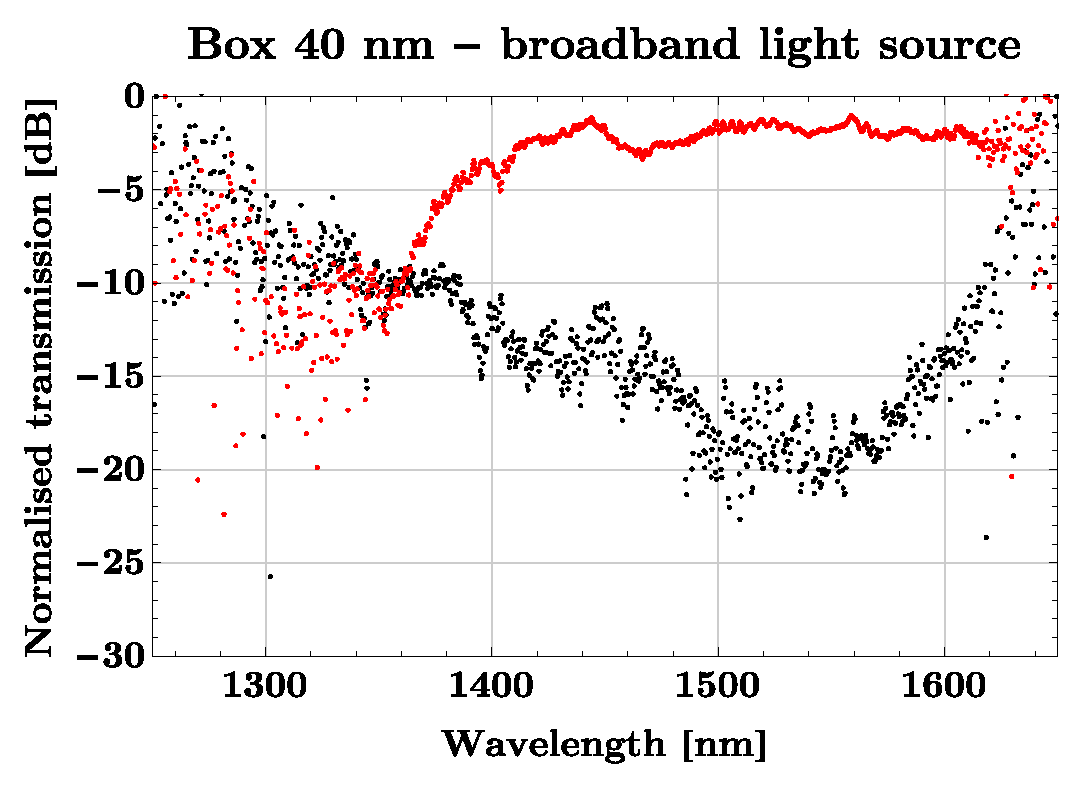
\includegraphics[width=0.6\textwidth]
        {fig/Kilde1Broadband/box40broadband.pdf}
    \caption{Data from box structure w. minimum feature size of 40 nm from a broadband light source. Black: Signal through upper output waveguide. Red: signal through lower output waveguide. This graph has no error bars, but all conclusions regarding the fabricated designs were based on data obtained by other light sources. The broadband light source yielded too noisy data, as seen on the plot.}
    \label{fig:Lightsource1Rep}
\end{figure}

As shown in the right side of Fig. \ref{fig:Lightsource1Rep}, the signal around 1550 nm in the lower output waveguide was significantly clearer, which can be explained by the intensity profile of the LED emitting more light with wavelength around 1500 nm. The structure is designed to split light into 1300 nm and 1550 nm. 

Because of too much noise, especially in the low wavelength range, it is difficult to draw a conclusion from the data.

The 1300 nm wavelength is too far from the 1430 nm peak wavelength that the LED produces, which means that the data obtained primarily is background noise.

\subsection{Multimeter light source}

The multimeter had 2 LEDs with peak wavelengths at 1310 nm and 1550 nm, respectively. Because the individual bandwidths of the light sources were too narrow to cover the wanted spectrum, we gathered data using both light sources and concatenated the data from the useful (non-noisy) regions to get a full wavelength spectrum. Specifically, the data points from 1200 nm to 1400 nm were measured with the light source peaking at 1310 nm. The data points from 1400 nm to 1650 nm were measured with the light source peaking at 1550 nm. The results are plotted in Fig. \ref{fig:transmissionkilde2conc}.

This method yielded more useful results than with the broadband LED. Even so, some of the data is still very noisy, which is why we have also measured using the supercontinuum light source.

\subsection{Supercontinuum light source}
The supercontinuum light source yielded significantly clearer results, as seen in Fig. \ref{fig:transmissionkilde3}. That said, the results are very comparable to the multimeter results from Fig. \ref{fig:transmissionkilde2conc}. 



\subsection{Multimeter light source plots}

\begin{figure}[H]
\begin{subfigure}[h]{0.50\textwidth}
        \centering
        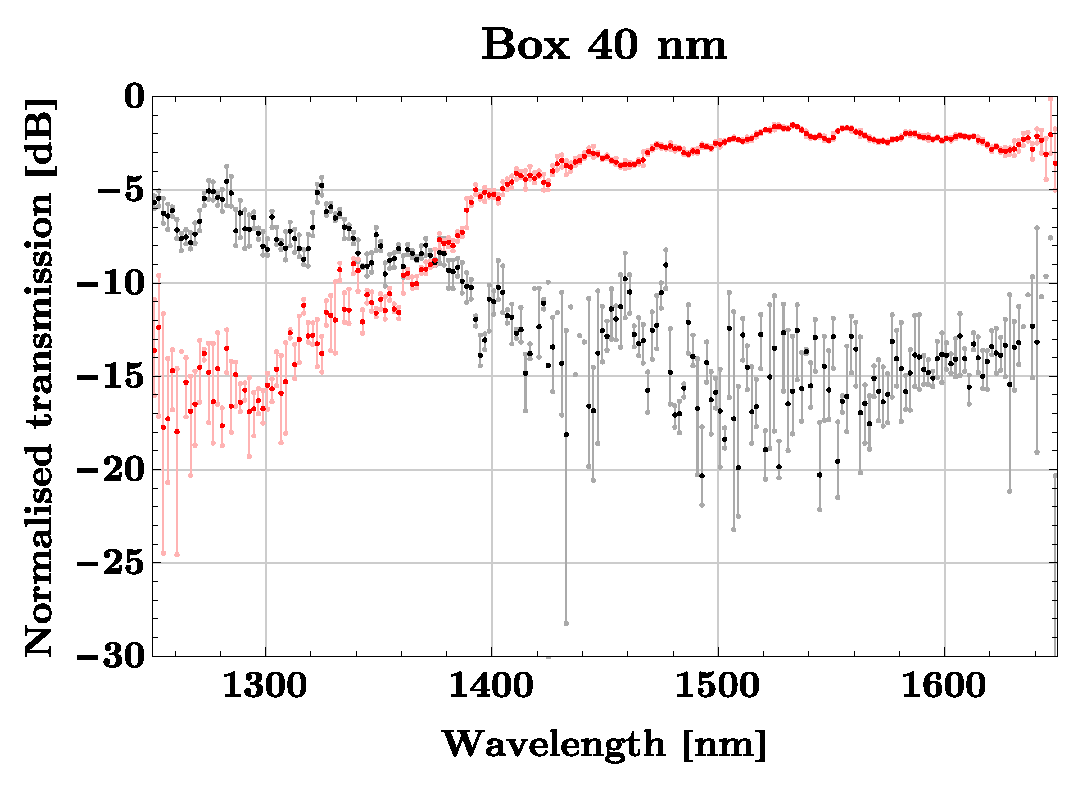
\includegraphics[width=1.0\textwidth]
        {fig/Kilde2Multimeter/box40multimeterconcatenated.eps}
        \caption{Transmission through the box structure with feature size 40 nm.}
    \end{subfigure}%
    ~ 
    \begin{subfigure}[h]{0.50\textwidth}
        \centering
        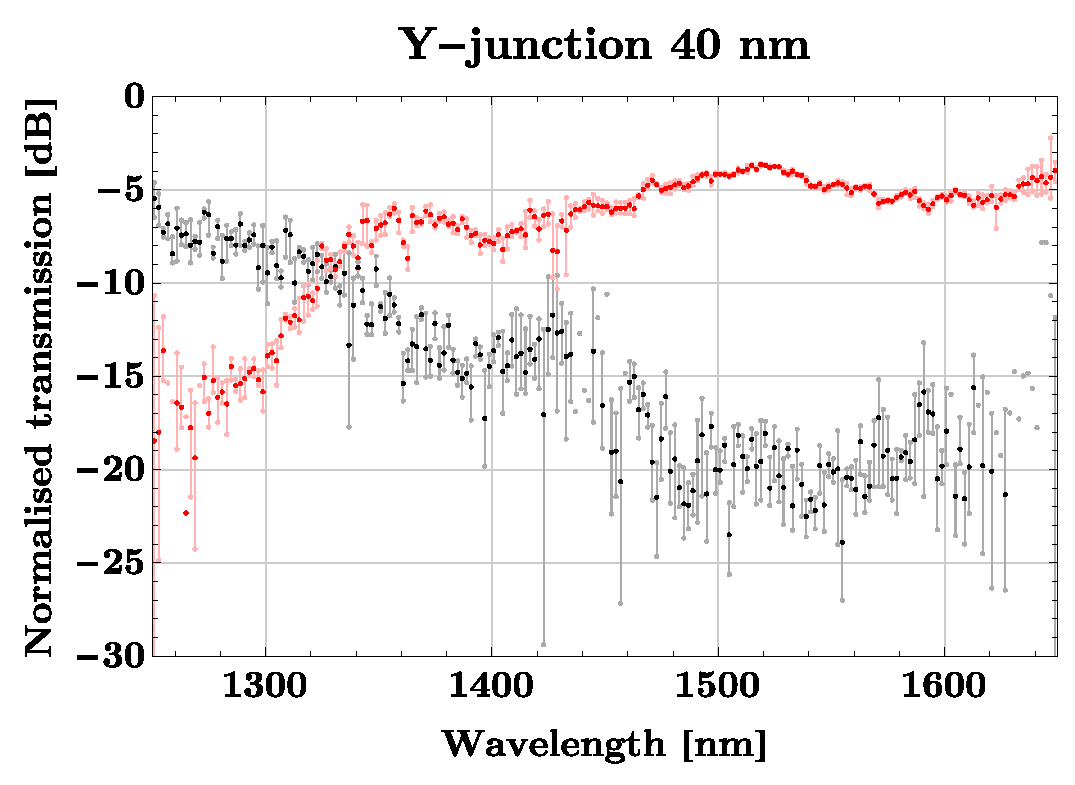
\includegraphics[width=1.0\textwidth]
        {fig/Kilde2Multimeter/yjunc40multimeterconcatenated.eps}
        \caption{Transmission through the Y-junction structure with feature size 40 nm.}
    \end{subfigure}
    
    \vspace{5 mm}
    
    
    \begin{subfigure}[h]{0.50\textwidth}
        \centering
        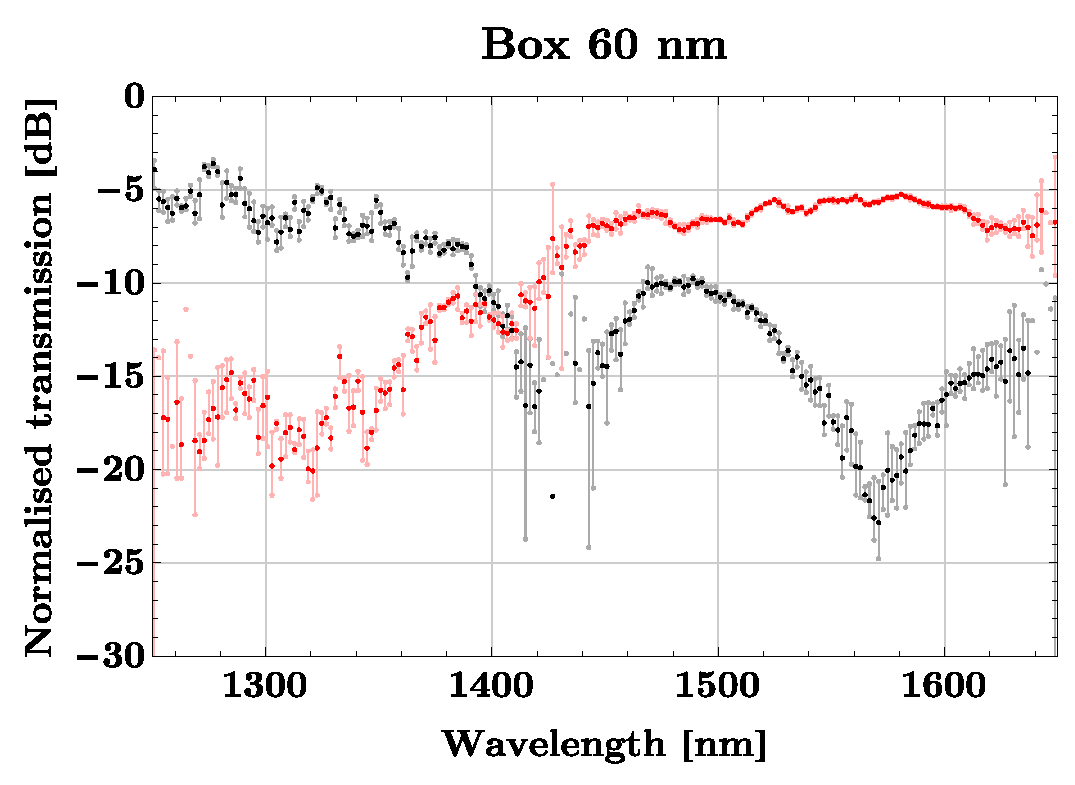
\includegraphics[width=1.0\textwidth]
        {fig/Kilde2Multimeter/box60multimeterconcatenated.eps}
        \caption{Transmission through the box structure with feature size 60 nm.}
    \end{subfigure}%
    ~ 
    \begin{subfigure}[h]{0.50\textwidth}
        \centering
        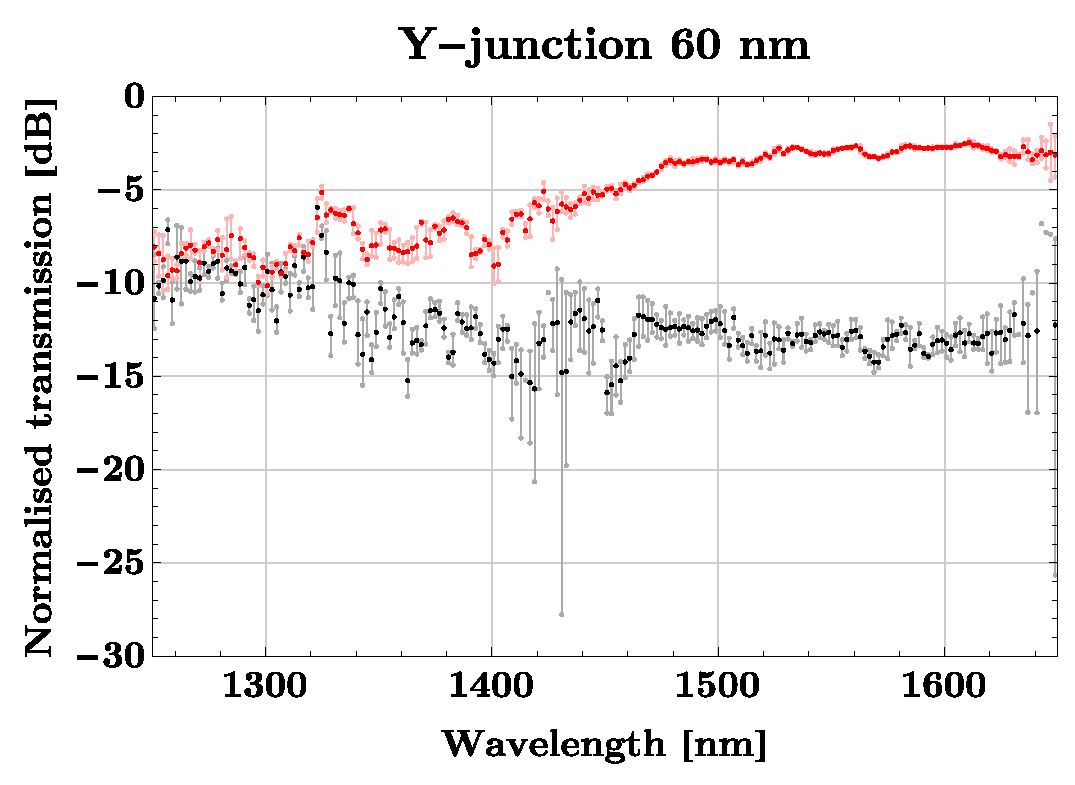
\includegraphics[width=1.0\textwidth]
        {fig/Kilde2Multimeter/yjunc60multimeterconcatenated.eps}
        \caption{Transmission through the Y-junction structure with feature size 60 nm.}
    \end{subfigure}
    
    \vspace{5 mm}
    
    \begin{subfigure}[h]{0.5\textwidth}
        \centering
        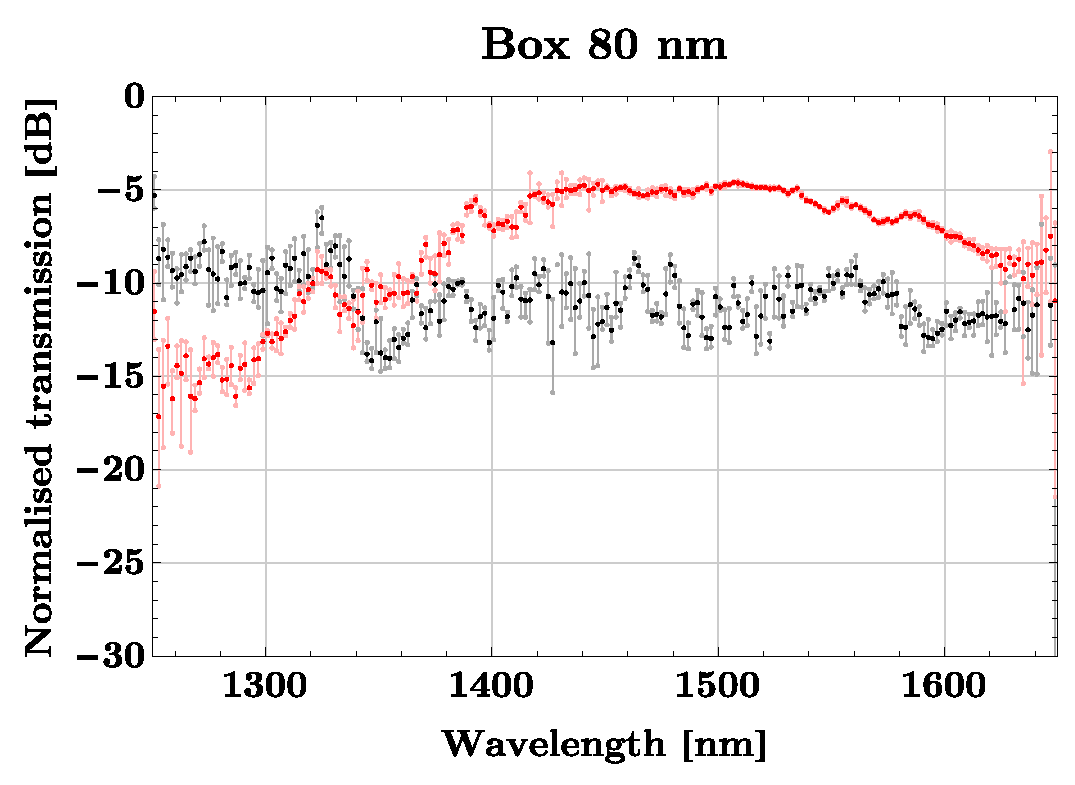
\includegraphics[width=1.0\textwidth]
        {fig/Kilde2Multimeter/box80multimeterconcatenated.eps}
        \caption{Transmission through the box structure with feature size 80 nm.}
    \end{subfigure}%
    ~ 
    \begin{subfigure}[h]{0.50\textwidth}
        \centering
        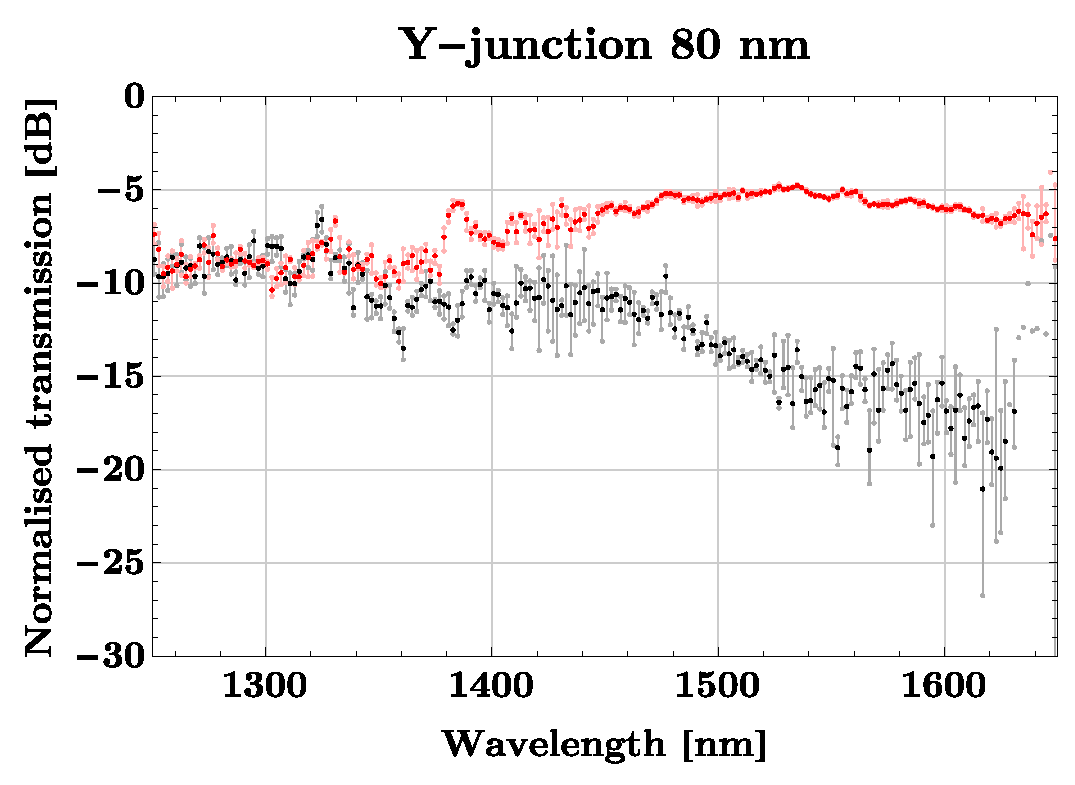
\includegraphics[width=1.0\textwidth]
        {fig/Kilde2Multimeter/yjunc80multimeterconcatenated.eps}
        \caption{Transmission through the Y-junction structure with feature size 80 nm.}
    \end{subfigure}
    \caption{Normalised transmission through fabricated structures. Black: Signal through upper output waveguide. Red: signal through lower output waveguide. The error bars mark maximum and minimum values obtained through 5-blocking (see the error bars subsection at page \pageref{sec:errorbars} for details). Measurements are obtained using the multimeter LEDs as light sources, see Table \ref{tablelightsources}.  The data are concatenated from two separate measurements; one measurement with the LED peaking at 1310 nm (data points in the interval  [1250, 1400] nm), one measurement with the LED peaking at 1550 nm (data points in the interval ]1400, 1650] nm).}
    \label{fig:transmissionkilde2conc}
    
\end{figure}

%

%Error bars are obtained through 5-blocking, see the Error Bars subsection (page \pageref{sec:errorbars}) for details.
\subsection{Supercontinuum light source plots}

\begin{figure}[H]
\begin{subfigure}[h]{0.50\textwidth}
        \centering
        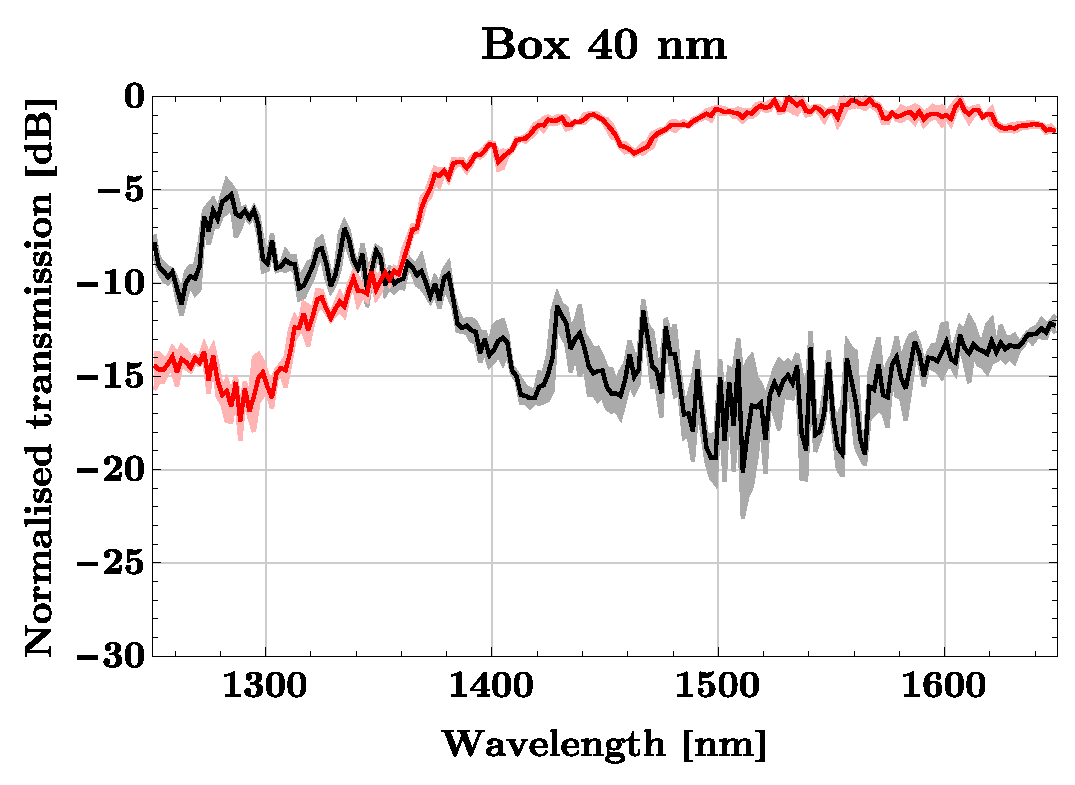
\includegraphics[width=1.0\textwidth]
        {fig/Kilde3Supercontinuum/box40supercontinuum.eps}
        \caption{Transmission through the box structure with feature size 40 nm.}
        \label{fig:transmissionkilde3_a}
    \end{subfigure}%
    ~ 
    \begin{subfigure}[h]{0.50\textwidth}
        \centering
        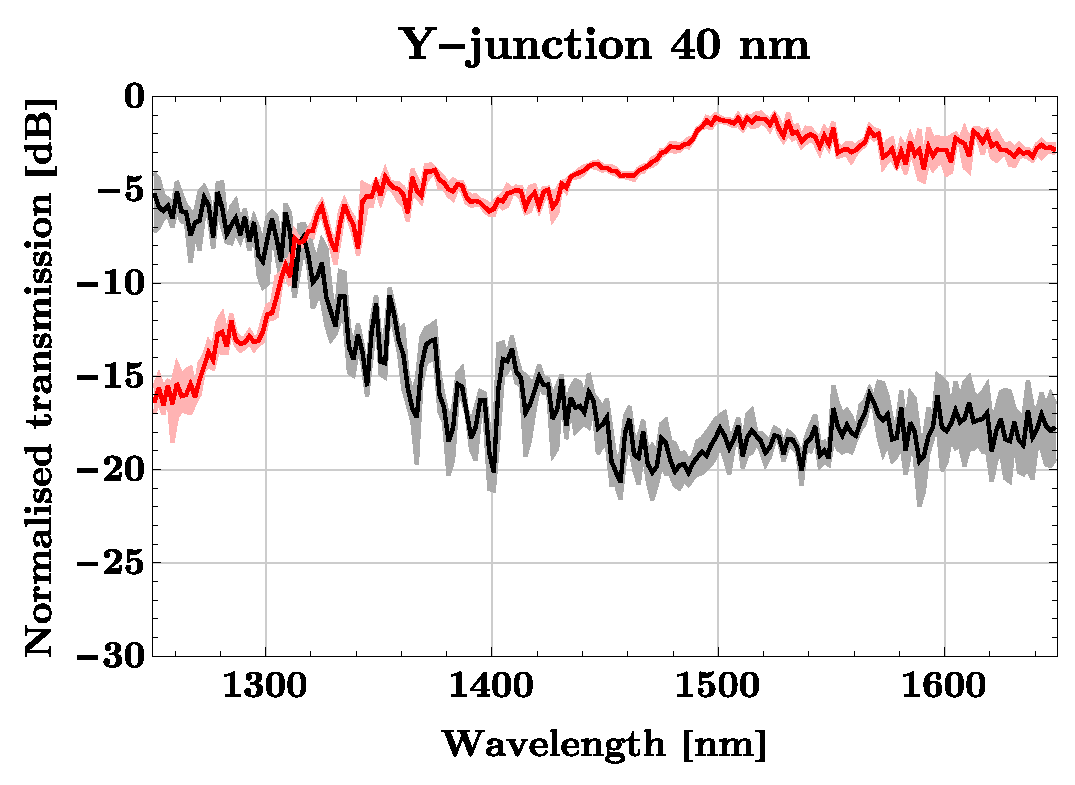
\includegraphics[width=1.0\textwidth]
        {fig/Kilde3Supercontinuum/yjunc40supercontinuum.eps}
        \caption{Transmission through the Y-junction structure with feature size 40 nm.}
        \label{fig:transmissionkilde3_b}
    \end{subfigure}
    
    \vspace{5 mm}
    
    
    \begin{subfigure}[h]{0.50\textwidth}
        \centering
        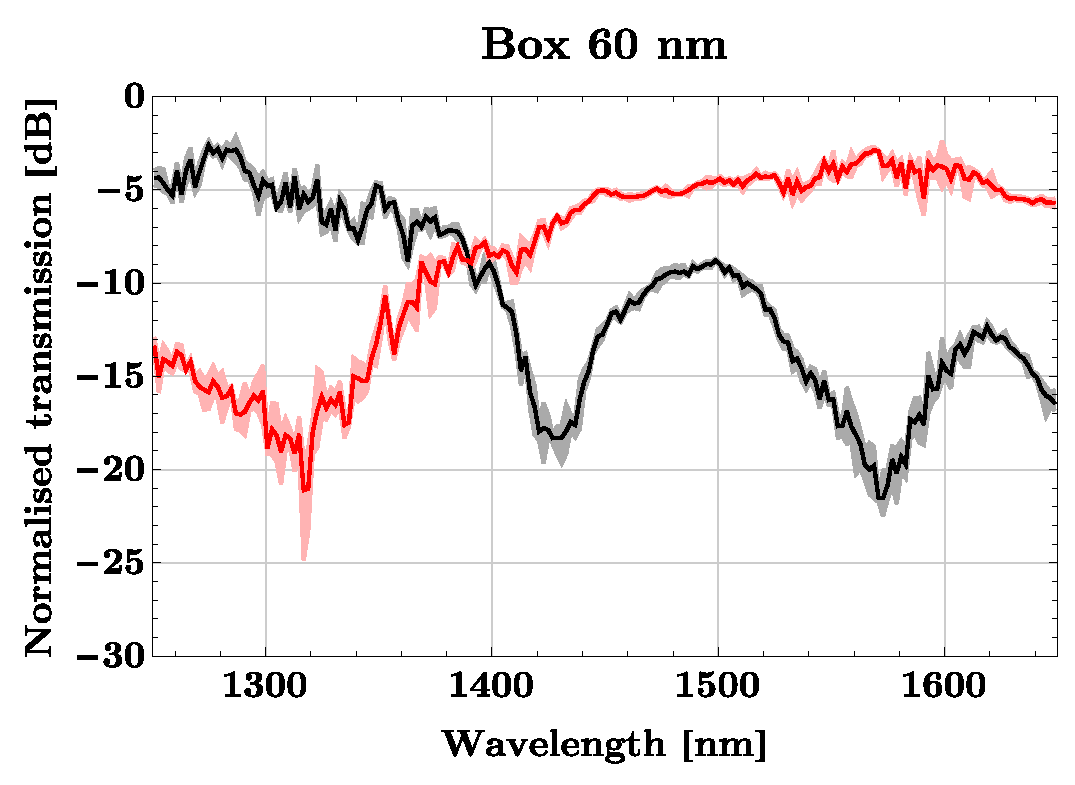
\includegraphics[width=1.0\textwidth]
        {fig/Kilde3Supercontinuum/box60supercontinuum.eps}
        \caption{Transmission through the box structure with feature size 60 nm.}
    \end{subfigure}%
    ~ 
    \begin{subfigure}[h]{0.50\textwidth}
        \centering
        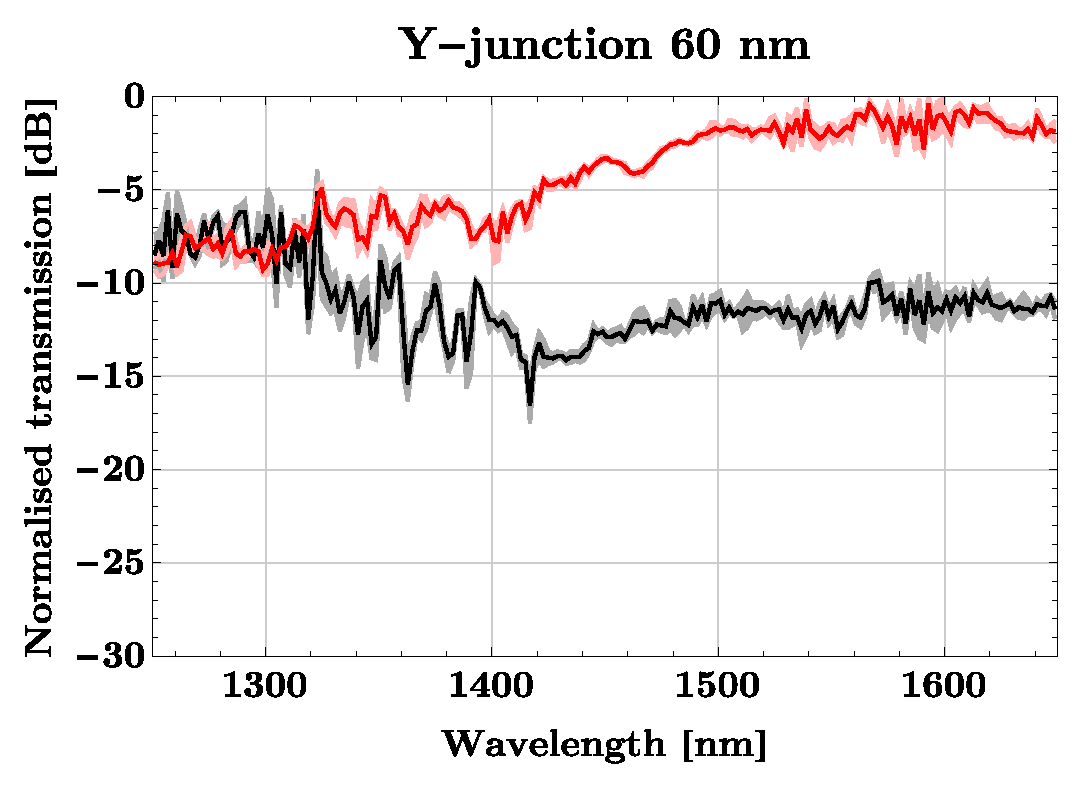
\includegraphics[width=1.0\textwidth]
        {fig/Kilde3Supercontinuum/yjunc60supercontinuum.eps}
        \caption{Transmission through the Y-junction structure with feature size 60 nm.}
    \end{subfigure}
    
    \vspace{5 mm}
    
    \begin{subfigure}[h]{0.5\textwidth}
        \centering
        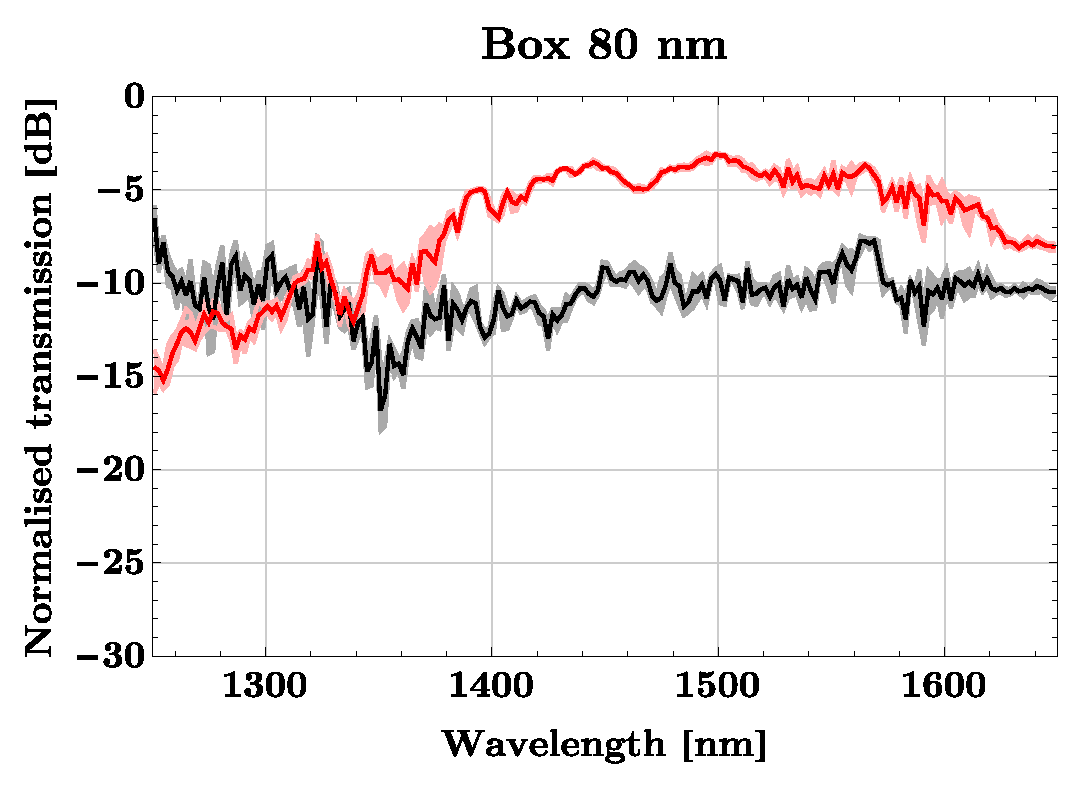
\includegraphics[width=1.0\textwidth]
        {fig/Kilde3Supercontinuum/box80supercontinuum.eps}
        \caption{Transmission through the box structure with feature size 80 nm.}
    \end{subfigure}%
    ~ 
    \begin{subfigure}[h]{0.50\textwidth}
        \centering
        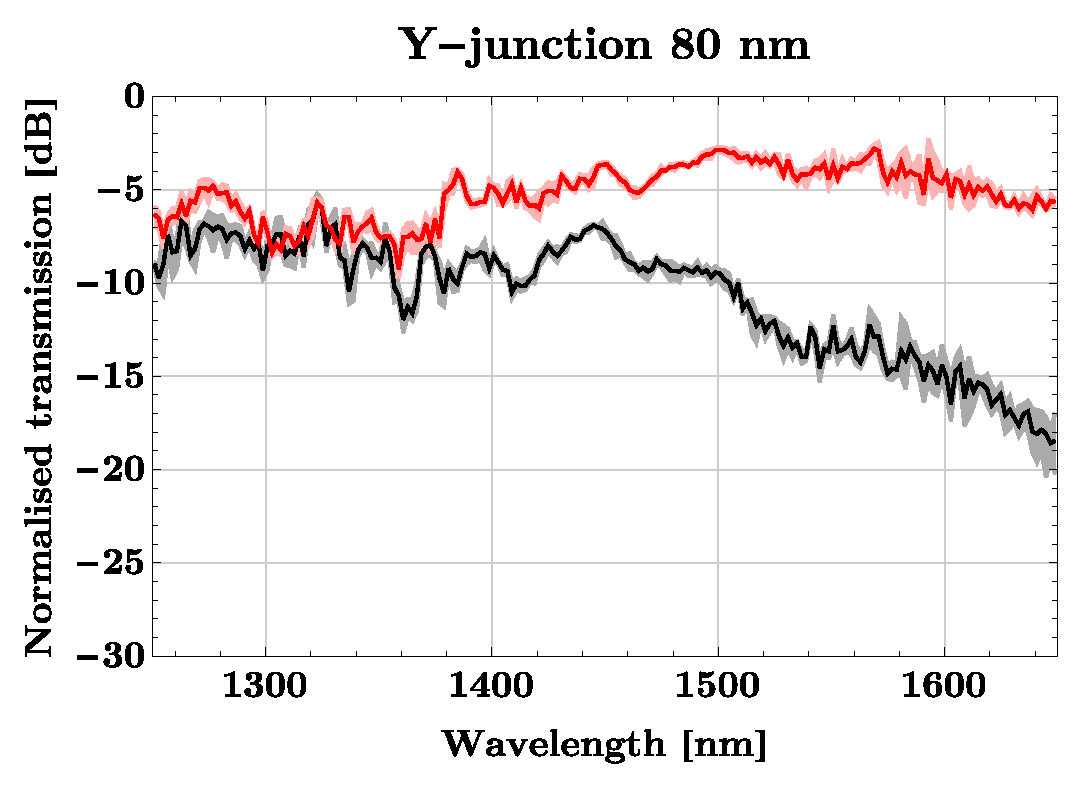
\includegraphics[width=1.0\textwidth]
        {fig/Kilde3Supercontinuum/yjunc80supercontinuum.eps}
        \caption{Transmission through the Y-junction structure with feature size 80 nm.}
    \end{subfigure}
    \caption{Normalised transmission through fabricated structures. Black: Signal through upper output waveguide. Red: signal through lower output waveguide. The shaded regions mark maximum and minimum values and are obtained through 5-blocking (See the Error Bars subsection  at page \pageref{sec:errorbars} for details). Measurements are obtained using the supercontinuum laser as a light source, see Table \ref{tablelightsources}.}
    \label{fig:transmissionkilde3}
    
\end{figure}

%The error bars mark maximum and minimum values (see the Error Bars subsection at page \pageref{sec:errorbars}) for details)
\subsection{Analysis and discussion}
This section concerns the plots in Fig. \ref{fig:transmissionkilde2conc} and \ref{fig:transmissionkilde3}. Also, peak insertion losses and graph intercepts are summarised in Table  \ref{table:supercontinuumBox} and Table  \ref{table:supercontinuumYjunction}.

\begin{table}[h]
\centering
    \begin{tabular}{|c|c|c|c|}
    \hline
    \textbf{Structure}      & \textbf{Box 40 nm} & \textbf{Box 60 nm} & \textbf{Box 80 nm} \\ \hline
    Peak insertion loss & $-$5 dB      & $-$5 dB      & $-$10 dB      \\
    (upper output) & ~         & ~         & ~         \\ \hline
    Peak insertion loss & $-$0 dB   & $-$5 dB      & $-$5 dB     \\
    (lower output) & ~         & ~         & ~         \\ \hline
    Peak crosstalk & $-$ 10 dB         & $-$ 8 dB       & $-$12 dB          \\  
    at wavelength      & 1350 nm   & 1380 nm   & 1320 nm     \\ \hline
    Crosstalk       & $-$15 dB  & [$-$16, $-$18] dB        & $-$12 dB          \\  
    at 1300 nm      & ~         & ~         & ~          \\  \hline
    Crosstalk       & [$-$15, $-$20] dB         & $-$17 dB         & $-$10 dB          \\  
    at 1550 nm      & ~         & ~         & ~          \\  \hline
    \end{tabular}
    \caption{Characteristics for box structures, read from the graphs for the supercontinuum light source in Fig. \ref{fig:transmissionkilde3}. Peak crosstalk is the intercept between the transmission graphs.}
    \label{table:supercontinuumBox}
\end{table}

\begin{table}[h]
\centering
    \begin{tabular}{|c|c|c|c|}
    \hline
    \textbf{Structure}      & \textbf{Y-junction 40 nm} & \textbf{Y-junction 60 nm} & \textbf{Y-junction 80 nm} \\ \hline
    Peak insertion loss & $-$5 dB      & [$-$10, $-$5] dB       & [$-$15, $-$10] dB      \\
    (upper output) & ~          & ~                 & ~                 \\ \hline
    Peak insertion loss & $-$3 dB      & [$-$5, $-$2] dB        &  $-$5 dB            \\
    (lower output) & ~          & ~                 & ~ \\ \hline
    Peak crosstalk & $-$7 dB         & $-$7 dB         & -          \\  
    at wavelength  & 1320 nm   & 1320 nm   & -     \\ \hline
    Crosstalk      & $-$12 dB         & $-$12 dB         & $-$8 dB   \\
    at 1300 nm     & ~         & ~         & ~           \\  \hline
    Crosstalk      & $-$17 dB         & $-$12 dB         & $-$12 dB  \\  
    at 1550 nm & ~         & ~         & ~          \\  \hline
    \end{tabular}
    \caption{Characteristics for Y-junction structures, read from the graphs for the supercontinuum light source in Fig. \ref{fig:transmissionkilde3}. Peak crosstalk is the intercept between the transmission graphs. The Y-junction with feature size 80 nm has no intercept; It just lowers all signal strengths. The lower output has a higher insertion loss, but since the device does not separate the signal, the device is meaningless.}
    \label{table:supercontinuumYjunction}
\end{table}

Across all designs, the performances are somewhat degraded, and sometimes differ greatly from the simulations. \\
\\
Among the six final designs, the box structure w. minimum feature size of 40 nm has the best performance. The high wavelengths are handled well: The peak insertion loss in the lower waveguide is rather suspiciously $-$0 dB, although read as $-$2 dB with the multimedia light source (see Fig. \ref{fig:transmissionkilde2conc}). This is comparable to the simulation results, while the upper waveguide nicely keeps the high-wavelength cross-talk at around $-$15 dB.
However, low wavelengths cause some trouble: The maximum output in the upper channel is lowered $-$4 dB compared to the simulations, and neither insertion losses nor transmission nor crosstalk values are particularly good.\\
\\
The best-performing Y-junction structure (feature size 40 nm) is comparable to the best-performing box structure with feature size 40 nm. Apparently manually altering the initial structure to a Y-junction did not remarkably improve the performance of the device.\\ 
\\
The other designs (feature sizes 60 nm and 80 nm) perform significantly worse than predicted by the simulations. In general it seems that larger minimum feature size yields worse performance. This was also the case in the simulations but only by $-$2 dB at most, see Table \ref{simtable}. We attribute this discrepancy to the fact that the designs w. larger minimum feature sizes also have larger shaded regions which were not possible to fabricate, as mentioned earlier. It seems that these shaded regions play an important role in the separation of the light.\\
\\
Since the intercept wavelength has been shifted $\approx$ 100 nm to the left for all the designs, it may be interesting to see how they perform for wavelengths below 1250 nm. But data for wavelengths lower than 1250 nm was not recorded in this project.\\



\section{Statistical analysis}

To evaluate the reproducibility of our results, we conducted three experiments to examine the uncertainties related to\\
\\
\textbf{A} manually positioning the fibres between measurements, \\
\textbf{B} recalibrating the polarisation crystal between measurements, \\
\textbf{C} recording transmission through a fabricated design after resetting both the fiber positions and polarisation. For all of these three experiments, the supercontinuum laser was used as a light source (see Table \ref{tablelightsources}).\\
\\
In \textbf{A}, we recorded the transmission through a reference waveguide. \\
In \textbf{B}, we recorded the transmission through a photonic crystal with a cut-off at $\approx$ 1560 nm.\\
In \textbf{C}, we recorded the transmission through a fabricated box structure with feature size 40 nm.

\subsection{Fiber positioning}

For every measurement recorded, the optical fibres must be positioned in order to get a signal through the current silicon structures. This contributes an uncertainty when normalising the signal from the designed structure with the reference waveguide. Five sets of measurements were performed with the supercontinuum laser on a reference waveguide. The supercontinuum has an intensity profile as seen in the appendix Fig. \ref{fig:superKref}. 
For each 5 data points at a given wavelength, the standard deviation of transmission is computed. As seen on Fig. \ref{fig:PositionError}, the standard deviations are on average 0.3 dB, and the highest deviation is around 1.2 dB. 

\begin{figure}[h!]
    \centering
    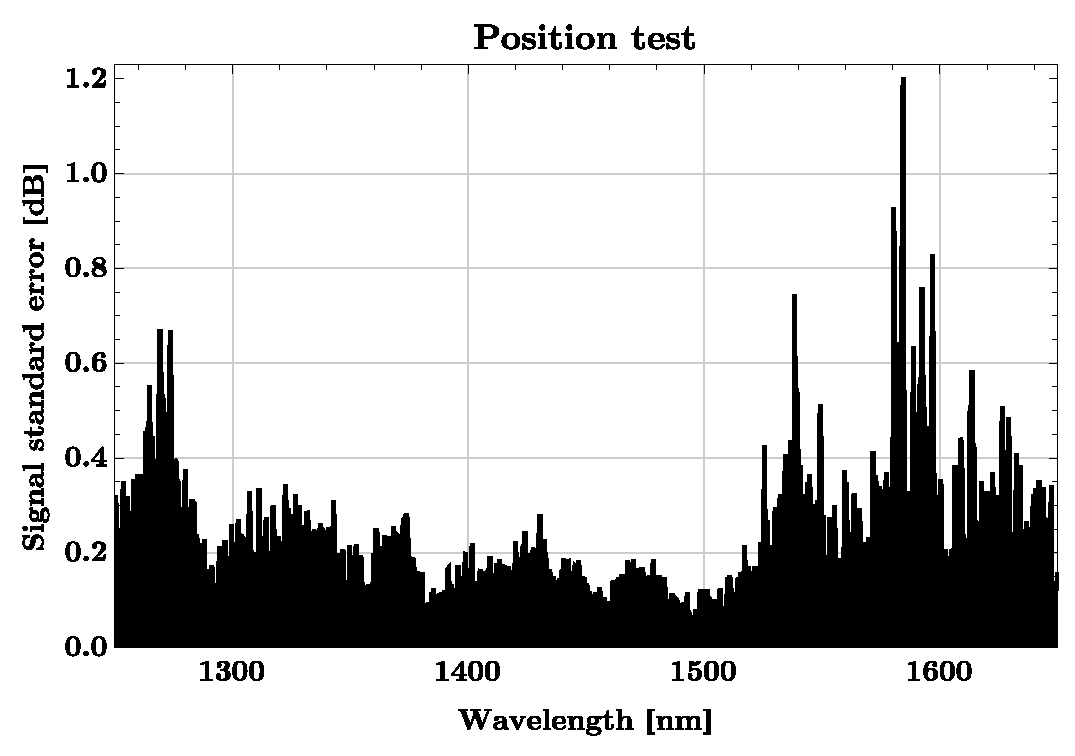
\includegraphics[width=0.8\textwidth]{fig/statistics/positiontest.eps}
    \caption{Standard deviation vs wavelength from positioning fibres.}
    \label{fig:PositionError}
\end{figure}

\subsection{Polarisation}

The intensity is highly dependent on the orientation of the twisters, so several measurements were gathered with the orientation of the twisters scrambled and then repositioned/optimised before each individual measurement. The results are shown in Fig. \ref{fig:PolarisationError}. \\

\begin{figure}[h!]
    \centering  
    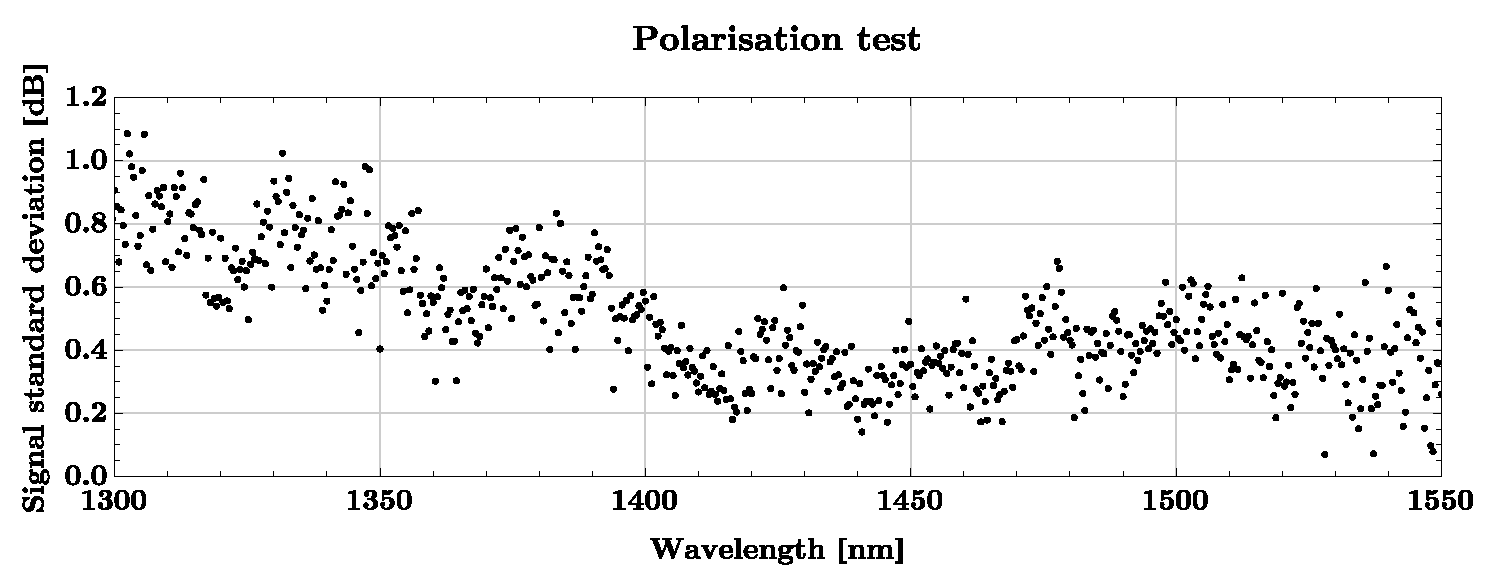
\includegraphics[width=\textwidth]{fig/statistics/polarisationtest2.eps}
    \caption{Standard deviation vs wavelength from setting polarisation with twisters.}
    \label{fig:PolarisationError}
\end{figure}

The measurements cover wavelengths below 1560 nm, since the photonic crystal cuts of higher wavelengths.

In Fig. \ref{fig:PolarisationError} we look at a section of the spectrum which is not dominated by background noise. We see that the standard deviation is no more than 2.0 dB, which suggests that the polarisation deviation is not the cause of the drastic fluctuations at wavelengths from the upper output waveguide within [1400, 1600] nm on Fig. \ref{fig:transmissionkilde3}.

\subsection{Consecutive readings of a single design}

The positions of the fibres and polarisation seem not to be the main cause of the observed fluctuations. As a final statistical analysis, we compute standard deviations from five sets of normalised data of the 40 nm box-formed design. Thus, five times we measured the signal through the design and reference waveguide.  Between each measurement set (of reference and design), the polarisation and position were scrambled and reset. Signal measurements can be seen in appendix Fig. \ref{fig:ConsecutiveFiveBox40}.

\begin{figure}[h!]
    \centering
    \begin{subfigure}[h!]{0.8\textwidth}
    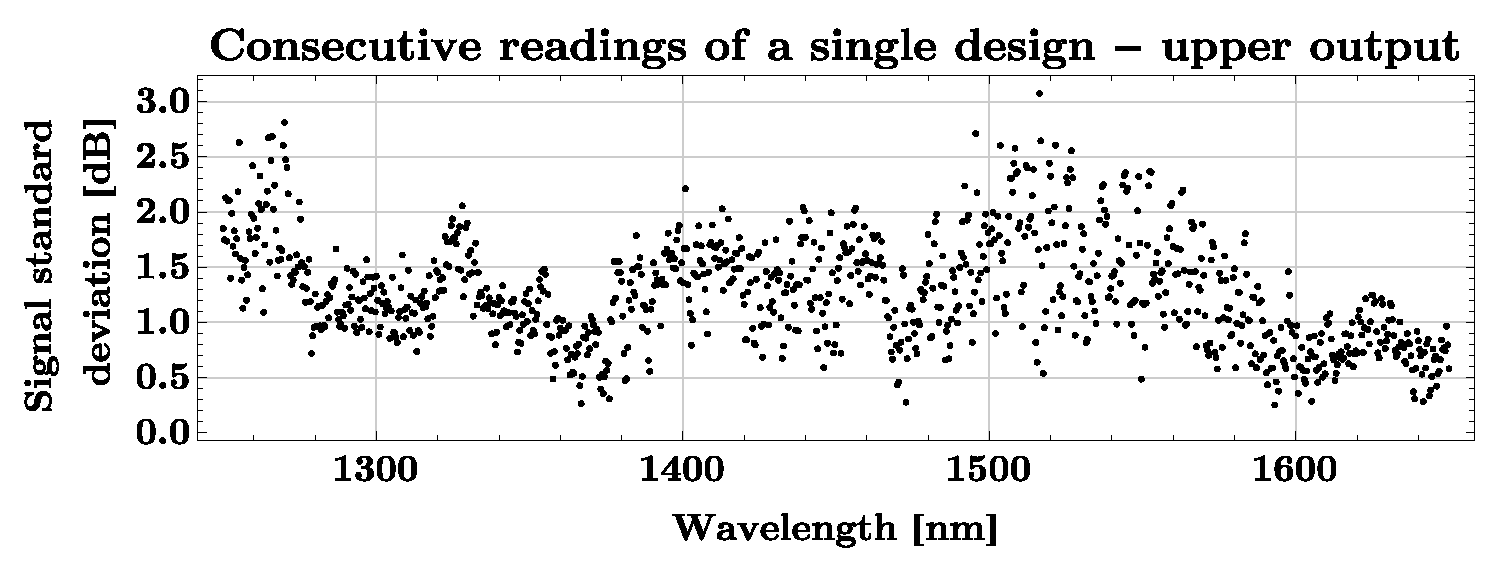
\includegraphics[width=\textwidth]{fig/statistics/ReproducibilityTestUpper.eps}
    \caption{Signal standard deviation in the upper output waveguide. This channel is intended to deliver light peaking at wavelength 1300 nm.}
    \label{fig:RepNorm1}
    \end{subfigure}

     \begin{subfigure}[h!]{0.8\textwidth}
    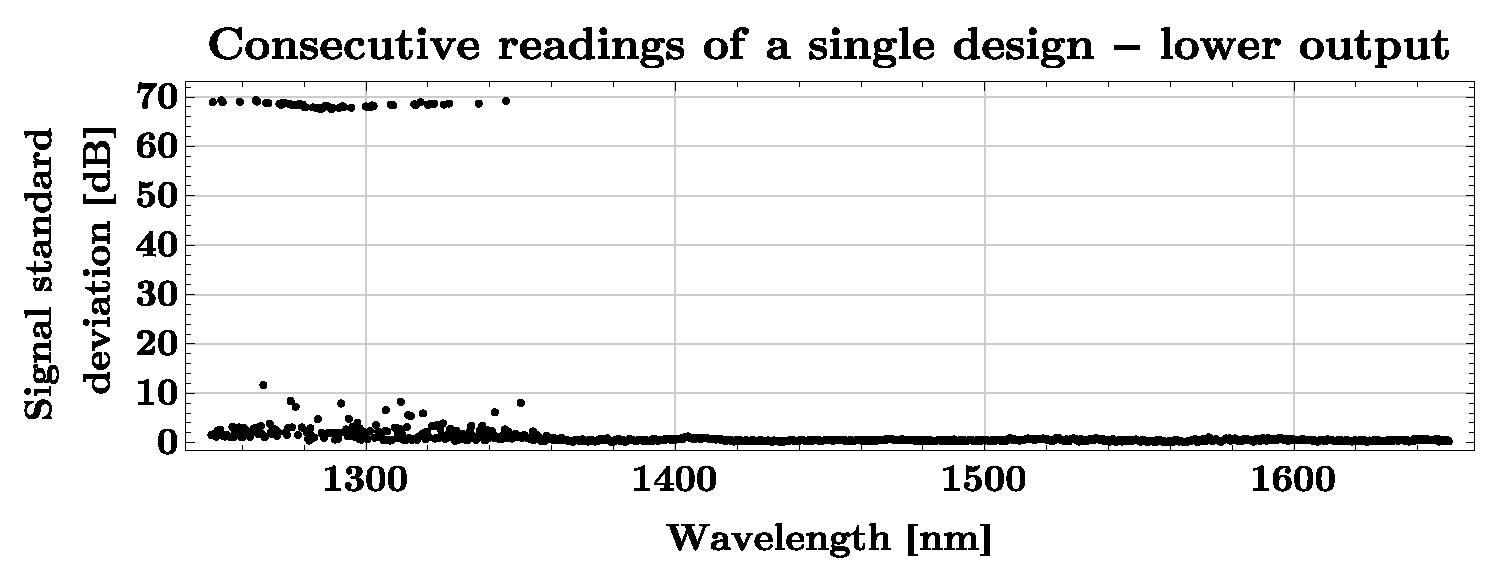
\includegraphics[width=\textwidth]{fig/statistics/ReproducibilityTestLower1250.eps}
    \caption{Signal standard deviation in the lower output waveguide. This channel is intended to deliver light peaking at wavelength 1550 nm.}
    \label{fig:RepNorm2}
    \end{subfigure}

     \begin{subfigure}[h!]{0.8\textwidth}
    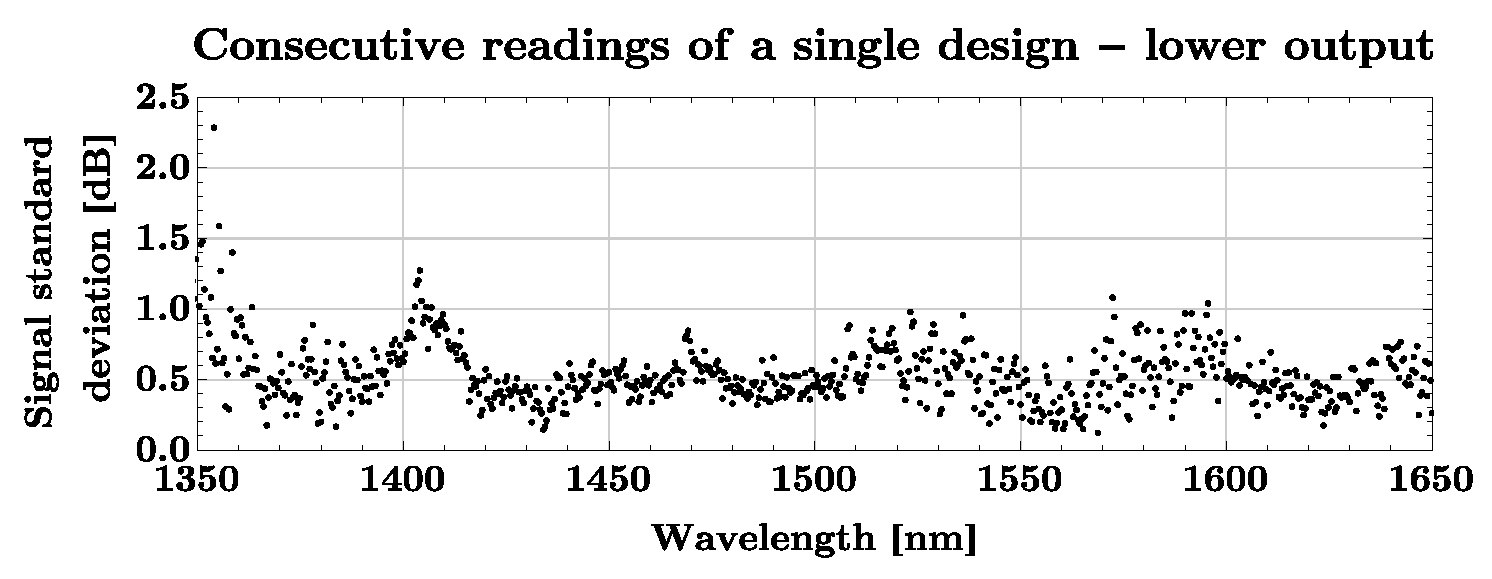
\includegraphics[width=\textwidth]{fig/statistics/ReproducibilityTestLower1350.eps}
    \caption{Section of the spectrum from Fig. \ref{fig:RepNorm2} not being dominated by background noise.}
    \label{fig:RepNorm3}
    \end{subfigure}
    
    \caption{Standard deviation vs wavelength of data from several measurements of the same structure.}
    \label{fig:RepNorm}
\end{figure}

From the measured data on Fig. \ref{fig:RepNorm1}, we read an average standard deviation around 1.5 dB and a maximum deviation around 3.1 dB for the signal through the upper waveguide. From the measured data on Fig. \ref{fig:RepNorm2} concerning the lower output waveguide, the maximum standard deviation is a whopping 70 dB. (This aberration is discussed in the next section.) If we look at the section without this disturbance on Fig. \ref{fig:RepNorm3} we see a standard deviation below 2.5 dB. 

\subsection{Analysis and discussion} 

From repositioning the fibres, the uncertainty (standard deviation) is on average 0.3 dB and at most 1.2 dB. From adjusting the polarisation, the standard deviation is on average 0.5 dB and at most 1.1 dB. \\
As these uncertainties should be independent (since we did not reposition the fibres during the polarisation test and vice versa), we calculate the combined uncertainty by adding the variances (that is, the squares of the standard deviations) and taking the square root. Thus we should expect the combined uncertainty to be on average 0.6 dB and 1.6 dB at most.\\ \vspace{1cm}

Looking at the statistical analysis of the lower waveguide  (Fig. \ref{fig:RepNorm3}), the uncertainty looks pretty much on the mark. The huge amount of noise at the low wavelengths (see Fig. \ref{fig:RepNorm2}) is caused by a single data sample, see Fig. \ref{fig:ConsecutiveFiveBox40} in Appendix. This sample has a signal intensity below the sensitivity of the OSA and can therefore be ignored. So it appears that repositioning the fibres and setting the polarisation are the main contributors to the uncertainty. 
\\
However, looking at the upper waveguide (Fig. \ref{fig:RepNorm1}) the deviations are much higher, on average 1.5 dB and peaking at 3.1 dB. This is actually on par with the large uncertainties on the upper waveguide in Fig. \ref{fig:transmissionkilde3_a} estimated by 5-blocking the data. (Note that the shaded regions mark maximum and minimum values. The distance from the average to a maximum or minimum value should be roughly two standard deviations.)\\

The change in uncertainty may be explained by the fact that the upper waveguide covers more low-intensity signal. Since the intensity of background noise is absolute, it should have a stronger relative influence on lower intensities. \\

%%%%%%%%%%%%%%%%%%Furthermore, the lower wavelengths have a higher dependency on the minimum feature size of the structure, meaning the binary division of shaded areas to either black or white effects the lower end of the spectrum more. \\ 

In summary, we estimate that the experimental results are reproducible within a margin of error (standard deviation) of 1.6 dB when looking at signal with high transmission, while the crosstalk-results are reproducible within a margin of error (standard deviation) of 3.1 dB. These estimates are quite pessimistic, but it is necessary when it is taken into account that the measurements are based on one of the structures. In order to lower the uncertainties, more experiments would have to be conducted.


\section{Conclusion}
We have shown that topology optimisation theoretically makes it possible to design silicon structures which demultiplex infrared light into 1300 nm wavelength and 1550 nm wavelength spectra. We obtained six designs with peak insertion losses at $-$0.83 dB or better, and crosstalk averaging at $-$15 dB and peaking at $-$6 dB (see Fig. \ref{fig:simplots}). 
The six fabricated structures, with the desired footprint, did not yield as satisfactory results, with peak insertion losses lowered to $-$5 dB in the 1300 nm region, and raised crosstalk throughout the 1250-1650 nm spectrum that we wanted to demultiplex. We attribute the lower performance to the fact that our designs require materials with permittivities between those of air and silicon. Curiously, the designs with the largest feature sizes seems to suffer from this, as they also feature the largest regions of materials with intermediate permittivites (See Fig. \ref{fig:BoxStructures} and \ref{fig:Y-juncStructures}).\\

For our best designs (see Fig. \ref{fig:transmissionkilde3_a} and \ref{fig:transmissionkilde3_b} with minimum feature sizes at 40 nm), the results are still very acceptable with peak insertion losses of $-$1 dB and $-$5 dB, in the 1550 nm spectrum and 1300 nm spetrum, respectively, and peak crosstalk at $-$10 dB. However, a statistical analysis suggests that the results are only reproducible within a margin of error (standard deviation) of 1.6 dB when looking at signal with high transmission, while the crosstalk-results are reproducible within a margin of error of 3.1 dB.

Our designs still match, and at some disciplines even outperform, those of our peers \cite{Stanford}. This shows the great potential of topology optimisation algorithms for being an efficient means of designing integrated optical components.




%\bibliographystyle{apsrev}
\newpage
\bibliography{bibliography.bib}

\newpage

\textbf{Appendix}

\begin{figure}[H]
    \centering
    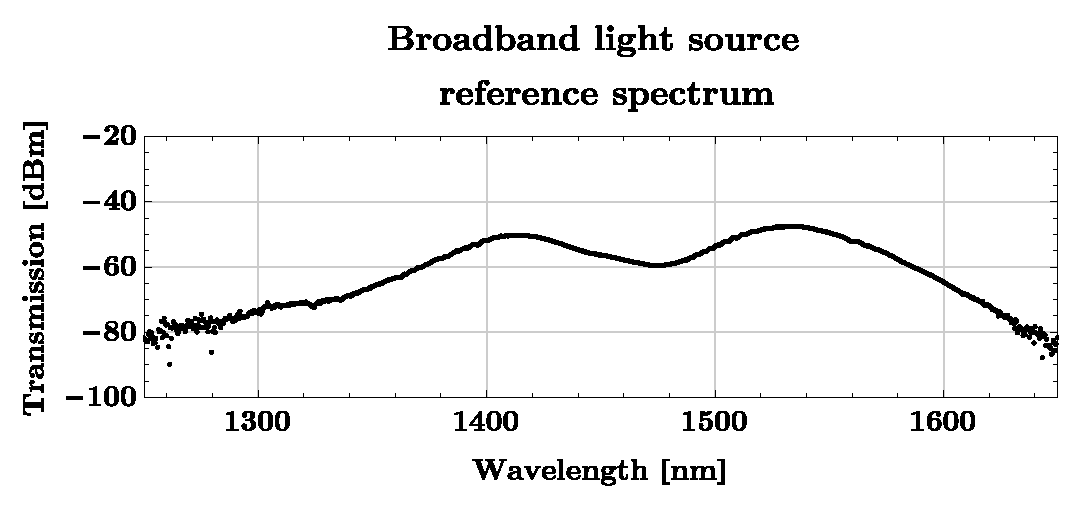
\includegraphics[width=0.7\textwidth]
    {fig/appendixrefplots/broadbandref.eps}
\vspace{-2mm}
    \caption{A typical reference spectrum for the broadband light source.}
    \label{fig:broadbandref}
\end{figure}

\vspace{-1.5cm}
\pagenumbering{gobble}

\begin{figure}[H]
    \centering
    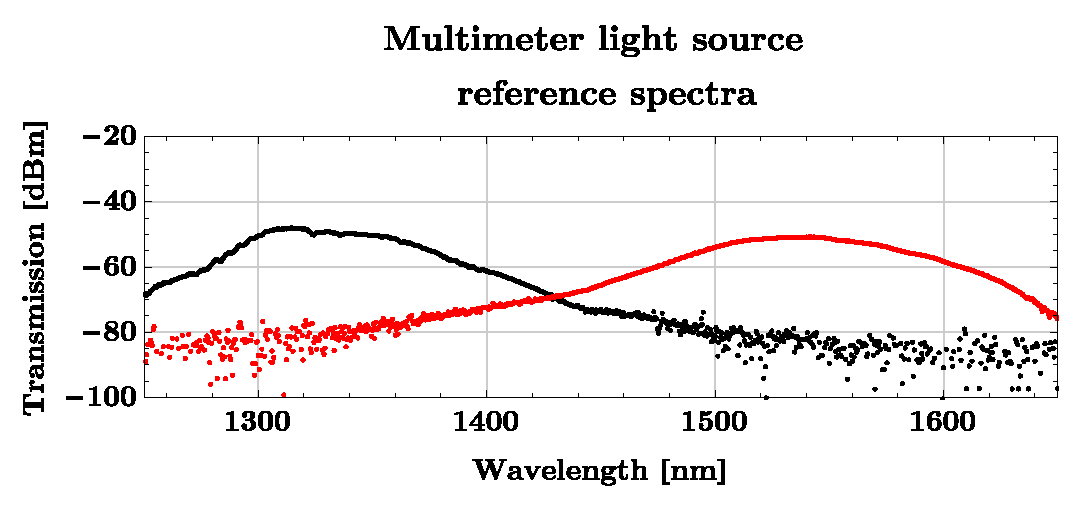
\includegraphics[width=0.7\textwidth]
    {fig/appendixrefplots/multimeterref.eps}
\vspace{-2mm}
    \caption{Typical reference spectra for the multimeter light source.}
    \label{fig:multimeterref}
\end{figure}

\vspace{-1.5cm}
\begin{figure}[H]
    \centering
    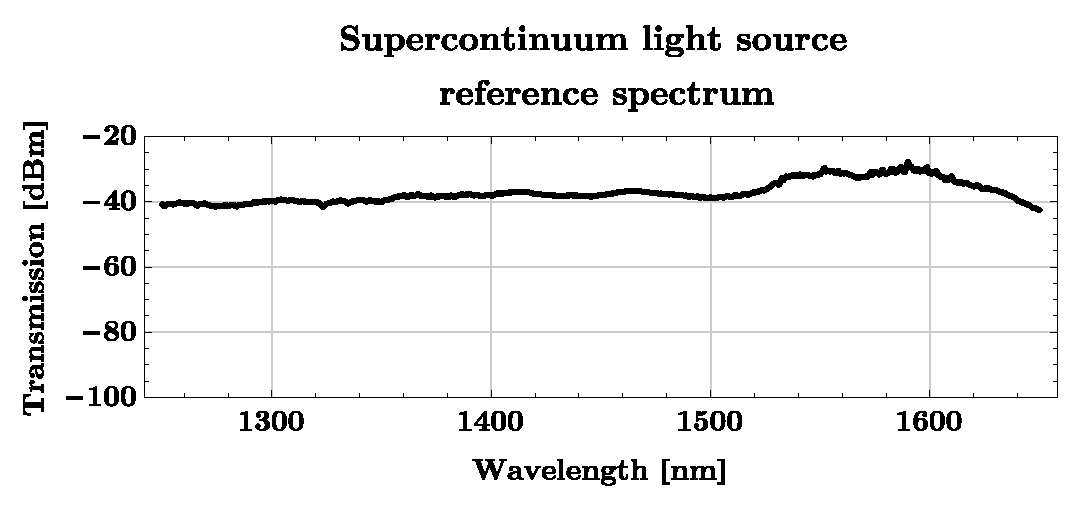
\includegraphics[width=0.7\textwidth]
    {fig/appendixrefplots/superKref.eps}
\vspace{-2mm}
    \caption{A typical reference spectrum for the supercontinuum light source.}
    \label{fig:superKref}
\end{figure}

\vspace{-1.5cm}
\begin{figure}[H]
    \centering
    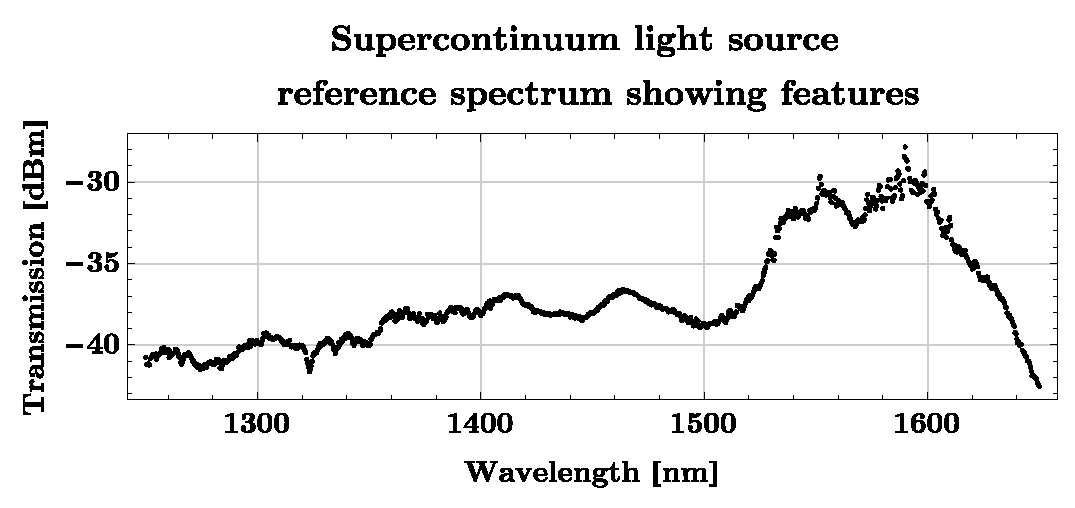
\includegraphics[width=0.7\textwidth]
    {fig/appendixrefplots/superKrefzoom.eps}
\vspace{-2mm}
    \caption{A typical reference spectrum for the supercontinuum light source showing the graph's features.}
    \label{fig:superKref}
\end{figure}


\begin{figure}[H]
    \centering
    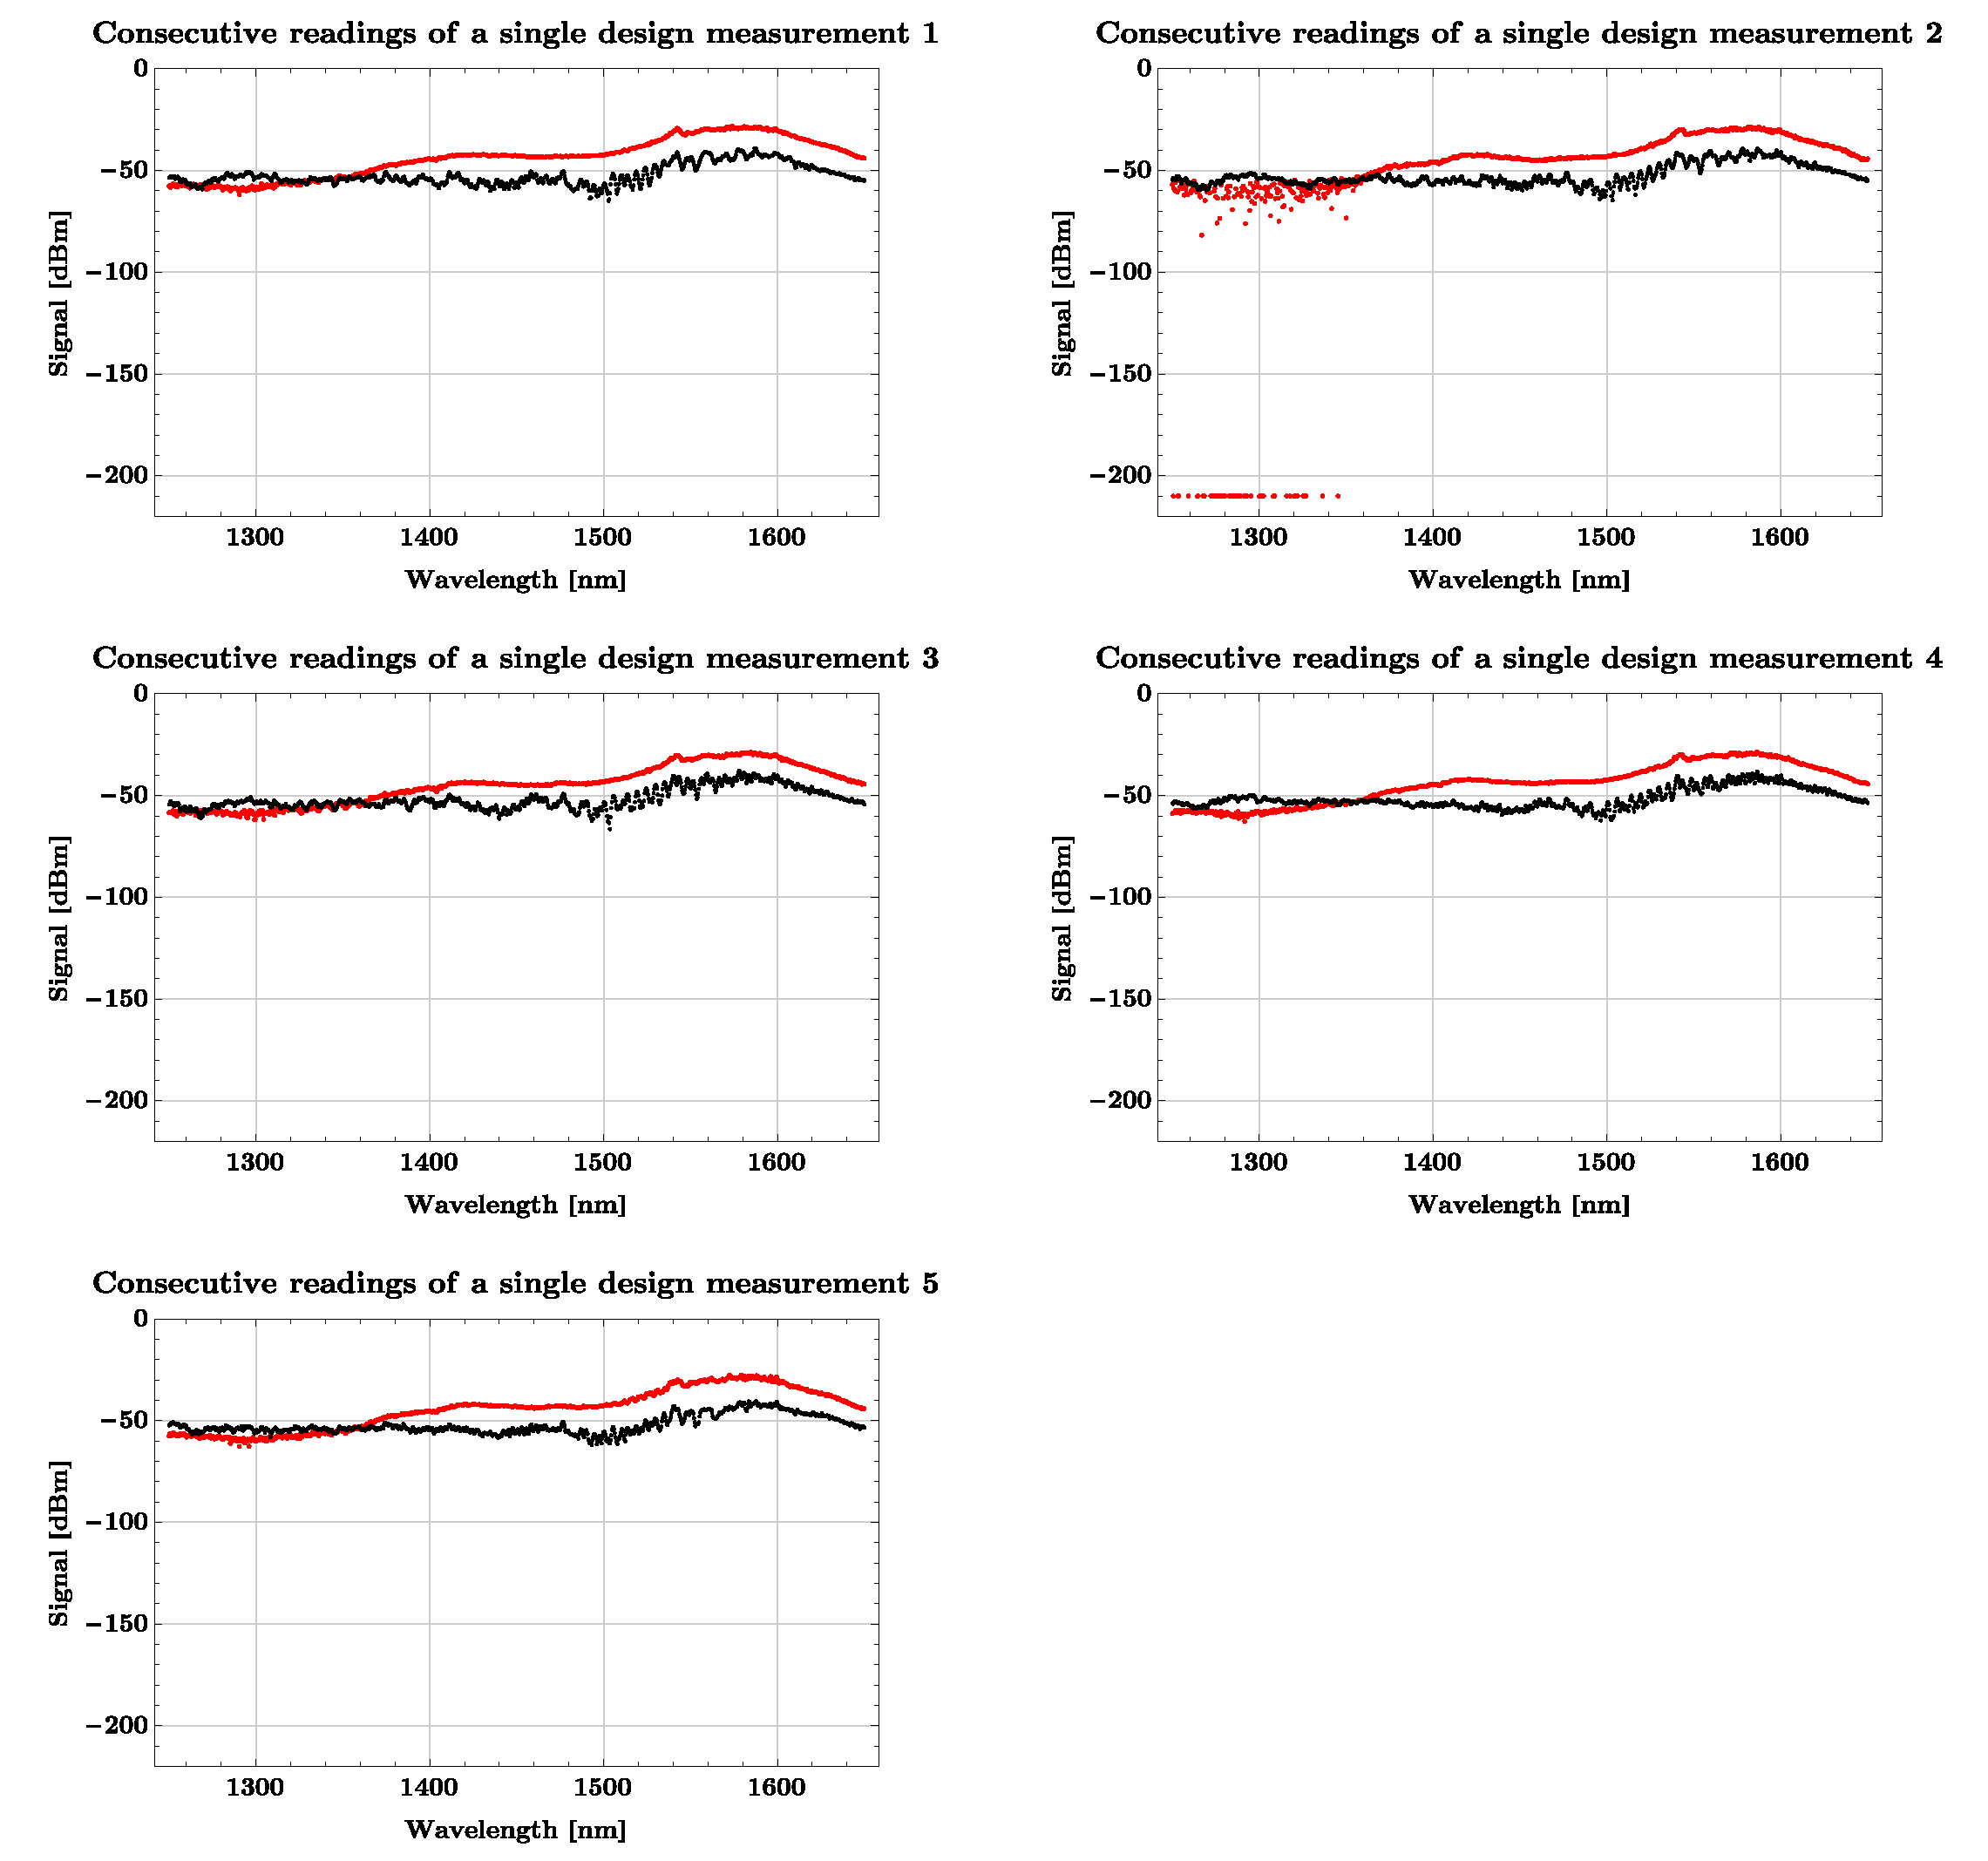
\includegraphics[width=1\textwidth]{fig/appendixrefplots/SignalPlots.eps}
    \caption{The sample of five measurements for consecutive readings on a single design (box 40 nm) with one sample having intensities below the sensitivity of the OSA, as seen on measurement 2.}
    \label{fig:ConsecutiveFiveBox40}
\end{figure}




\end{document}
